\documentclass[12pt]{iopart}
\usepackage{iopams}  
\usepackage{braket,graphicx,amsmath}
\usepackage[hidelinks]{hyperref}
\usepackage[margin=2cm]{geometry}
\bibliographystyle{unsrt}
\begin{document}

\title{Supplementary Materials for ``Frustration shapes multi-channel Kondo physics: a star graph perspective"}

\author{Siddhartha Patra$^1$, Abhirup Mukherjee$^1$, Anirban Mukherjee$^1$, N. S. Vidhyadhiraja$^4$, A. Taraphder$^5$ and Siddhartha Lal$^1$}
\eads{\mailto{sp14ip022@iiserkol.ac.in}, \mailto{am18ip014@iiserkol.ac.in}, \mailto{mukherjee.anirban.anirban@gmail.com}, \mailto{raja@jncasr.ac.in}, \mailto{arghya@phy.iitkgp.ernet.in}, \mailto{slal@iiserkol.ac.in}}

\address{$^1$Department of Physical Sciences, Indian Institute of Science Education and Research-Kolkata, W.B. 741246, India}

\address{$^4$Theoretical Sciences Unit, Jawaharlal Nehru Center for Advanced Scientific Research, Jakkur, Bengaluru 560064, India}

\address{$^5$Department of Physics, Indian Institute of Technology Kharagpur, Kharagpur 721302, India}

\date{\today}

\section{Additional Properties of the Star Graph}

\subsection{Partition function of the zero-mode fixed-point Hamiltonian, in the presence of a magnetic field}
The zero-mode approximation of the fixed-point Hamiltonian is a star graph Hamiltonian:
\begin{eqnarray}
	H = J^* \vec{S_d}\cdot\vec{s}_\text{tot}
\end{eqnarray}
where \(\vec s_\text{tot} = \sum_l \vec s_l\) is the total spin operator for all the channels. We insert a magnetic field that acts only on the impurity and then attempt to diagonalize the Hamiltonian.
\begin{eqnarray}
	\label{stargraph_field_hamiltonian}
	H(h) = J^* \vec{S_d}\cdot\vec{s}_\text{tot} + h S_d^z
\end{eqnarray}
The Hamiltonian commutes with \(s_\text{tot}^2\):
\begin{eqnarray}
	\hspace*{-20pt}\left[s_\text{tot}^2, H(h)\right] &= \left[\sum_{i=x,y,z}{s^i_\text{tot}}^2, J^* \sum_{i=x,y,z} S_d^i s^i_\text{tot}\right] = \sum_{i,j}J^* S_d^i \left\{s_\text{tot}^i, \left[s_\text{tot}^i,s_\text{tot}^j\right]\right\} = \sum_{i,j}J^* S_d^i \left\{s_\text{tot}^i, i \epsilon^{ijk}s^k_\text{tot}\right\}\nonumber\\
							 &= 0
\end{eqnarray}
This means the Hamiltonian is already block-diagonal in the quantum number \(s_\text{tot}\). Let us represent the quantum number of \(s_\text{tot}^z\) by \(m\). For a particular \(s_\text{tot}\), \(m\) can take values from the set \(\left[-s_\text{tot}, s_\text{tot}\right] \). The spin \(S_d^z\) can also take values \(\pm \frac{1}{2}\). From now on, we will assume we are in the subspace of a particular \(s_\text{tot} = M\), so we will ignore that quantum number and write the kets simply as \(\ket{S_d^z, m}\). So, the notation \(\ket{\uparrow,-1}\) means the state with \(S_d^z = \frac{1}{2}\) and \(m = -1\). We will now show that even inside the block of \(2\times s_\text{tot}\) (or \(2\times s_\text{tot} + 1\), depending on where it is odd or even) defined by a particular value of \(s_\text{tot}\), the Hamiltonian actually separates into decoupled \(2\times 2\) blocks. To see why, first note that the terminal states \(\ket{\downarrow, -M}\) and \(\ket{\uparrow, M}\) are already eigenstates, because they cannot scatter (the impurity can only flip down, and this would require the bath to flip up, but \(s^z_\text{tot}\) is already at its maximum value \(M\)). The other \(2M - 2\) states can be organized into \(2\times 2\) blocks formed by the states \(\ket{\uparrow, m}\) and \(\ket{\downarrow, m+1}\) for \(m \in \left[-M, M-1\right] \). The fact that this block does not interact with the other blocks can be observation: if there was some other state which when acted upon by the Hamiltonian gave a non-zero projection on \(\ket{\uparrow, m}\), it would have to come from \(S_d^z = \downarrow\), and this would mean the bath spin would have had to flip down. This means the bath spin in that state would have to be \(m+1\), and that is precisely the other state in the block. 

Defining \(\epsilon^h_m = \frac{1}{2}\left(Jm + h\right) \) and \(x^M_m = M(M+1) - m(m+1)\), the \(2\times 2\) blocks can be written as
\begin{eqnarray}
	H_m = \begin{pmatrix} \epsilon^h_m & \frac{J}{2}\sqrt{x^M_m} \\ \frac{J}{2}\sqrt{x^M_m} & -\left( \epsilon^h_m + J/2 \right)   \end{pmatrix} 
\end{eqnarray}
The eigenvalues are 
\begin{eqnarray}
	\label{eigenvalue}
	\lambda_{m, \pm}^{M, h} = \frac{1}{2}\left[-J/2 \pm \sqrt{J^2/4 + J^2 x_m^M + 4\epsilon^h_m\left(\epsilon^h_m + J/2\right) }\right] = -J/4 \pm \sqrt{J^2x^M_m/4 + \alpha^2}
\end{eqnarray}
where \(\alpha = \epsilon^h_m + J/4\).
The eigenvalues of the terminal states are \(\pm\epsilon^h_{\pm M}\). For \(h = 0\), the ground state subspace is \(K-\)fold degenerate and is formed by the negative solutions of eq.~\ref{eigenvalue}. This common \(K-\)fold degenerate eigenvalue is \(-J(M+1)/2\).
The eigenstates for each value of \(M,m\) in the \(J=M-\frac{1}{2}\) sector are given by
\begin{eqnarray}
	\fl \ket{M-\frac{1}{2},m+\frac{1}{2},M} =\mathcal{C}_\pm \ket{\uparrow, M, m} \pm \sqrt{1 - \mathcal{C}_\pm^2} \ket{\downarrow, M, m+1}, ~ ~ \mathcal{C}_\pm = \frac{J\sqrt{x_m^M}/2}{\sqrt{J^2 x_m^M/4 + \left(\alpha \mp \sqrt{\alpha^2 + J^2 x_m^M/4}\right)^2 }}
\end{eqnarray}
The partition function is given by
\begin{eqnarray}
	Z(h) = \sum_{M=M_\text{min}}^{M_\text{max}}\left[\sum_{m=-M, \atop{m\in \mathbb{Z}}}^{M-1}2e^{\beta J/4}\cosh \beta\sqrt{J^2x^M_m/4 + \alpha^2} + 2e^{-\beta JM/2}\cosh \beta h/2\right]
\end{eqnarray}
where \(M_\text{max} = K/2\) for a \(K-\)channel Kondo model, and \(M_\text{min} = 0\)  if \(K\) is even, otherwise \(1/2\). This is yet not the complete partition function, because we have not accounted for the possibility that there multiple subspaces of \(M\). For example, the \(K=3\) case states can be obtained by adding the third spin-half onto the states \(S=0,1\). \(S=0\) gives \(s_\text{tot}=1/2\) and \(S=1\) gives \(s_\text{tot} = 1/2, 3/2\). So, \(s_\text{tot} = 1/2\) appears twice. These two subspaces are actually orthogonal, because the quantum numbers for the individual channels are different. We need to count the number of instances of a particular subspace \(s_\text{tot}=M\). It turns out that this number is given by \(r^K_M = {}^{K-1}C_{K/2 - M}\), which means the correct partition function is
\begin{eqnarray}
	Z(h) &=\sum_{M=M_\text{min}}^{M_\text{max}}r^K_M\left[\sum_{m=-M, \atop{m\in \mathbb{Z}}}^{M-1}2e^{\beta J/4}\cosh \beta\sqrt{J^2x^M_m/4 + \alpha^2} + 2e^{-\beta JM/2}\cosh \beta h/2\right]
\end{eqnarray}

\subsection{Features of the polarised ground-states}
Of particular importance within the ground-state subspace are the zero-field maximally-polarised states, obtained by choosing \(M = \frac{K}{2}, m + \frac{1}{2}= \pm \left( M - \frac{1}{2} \right) =\pm \frac{1}{2}\left(K-1\right)\):
\begin{eqnarray}
	\fl \ket{J=\frac{K-1}{2},J^z= \frac{\sigma}{2}\left(K-1\right),s_\text{tot}=\frac{K}{2}} = \frac{1}{\sqrt{1 + K}} \ket{\sigma}_d\otimes\ket{s_\text{tot}^z=\sigma(\frac{K}{2}-1)} - \frac{\sqrt K}{\sqrt{1 + K}}\ket{\bar\sigma}_d\otimes\ket{s_\text{tot}^z=\sigma\frac{K}{2}},
\end{eqnarray}
where \(\sigma\) can take values \(\pm 1\) and \(\ket{\sigma}_d\) represents the up and down configurations of the impurity spin. The state \(\ket{s_\text{tot}^z=\frac{\sigma K}{2}}\) has all the bath spins pointing in the \(\sigma-\)direction: \(\ket{s_\text{tot}^z=\frac{\sigma K}{2}} = \ket{\sigma,\sigma,\ldots,\sigma} (\sigma=\uparrow \text{ or }\downarrow)\), where the notation is such that a particular symbol (say \(\uparrow\)) at the \(i^\text{th}\) position indicates the configuration of the \(i^\text{th}\) channel. The other state \(\ket{s_\text{tot}^z=\sigma(\frac{K}{2} - 1)}\) can be obtained by flipping any one out of the \(K\) spins in the previous state \(\ket{s_\text{tot}^z=\frac{\sigma K}{2}}\), leading to the normalised state \(\ket{s_\text{tot}^z=\sigma(\frac{K}{2} - 1)} = \frac{1}{\sqrt K}\ket{\bar\sigma,\sigma,\ldots,\sigma} + \frac{1}{\sqrt K}\ket{\sigma,\bar\sigma,\ldots,\sigma} + \ldots + \frac{1}{\sqrt K}\ket{\sigma,\sigma\ldots,\bar\sigma}\), a linear combination of all possible states with the spin of one channel in \(\bar\sigma(=-\sigma)\) direction and all other channels remaining in the \(\sigma\) direction. With these in mind, the polarised state can be cast in the more explicit form
\begin{eqnarray}
	\fl \ket{J^z= \frac{\sigma}{2}\left(K-1\right)} = \frac{1}{\sqrt{K(1 + K)}} \left[\ket{\sigma}_d\otimes\left(\ket{\bar\sigma,\sigma,\ldots,\sigma} + \ket{\sigma,\bar\sigma,\ldots,\sigma} + \ldots + \ket{\sigma,\sigma\ldots,\bar\sigma}\right) - K\ket{\bar\sigma}_d\otimes \ket{\sigma,\sigma,\ldots,\sigma}\right].\label{polarised-state}\qquad
\end{eqnarray}

In order to make the frustration faced by the impurity manifest, we now rewrite these polarised states in the form of superpositions of zero magnetisation singlet states. Let us define the singlet state \(\ket{\text{SS}_{d,l}} = \frac{1}{\sqrt 2}\left(\ket{\uparrow}_d\ket{\downarrow}_l - \ket{\downarrow}_d\ket{\uparrow}_l\right),l\in[1,K]\), between the impurity spin and the \(l^\text{th}\) channel, where \(\ket{\cdot}_l\) represents the configuration of the spin in the \(l^\text{th}\) channel. The polarised states can then be written as
\begin{eqnarray}
	\fl \ket{J^z= \frac{\sigma}{2}\left(K-1\right)} = \frac{1}{\sqrt{K(1 + K)}} \sum_{l=1}^K\ket{\sigma}_d\otimes\left[\ket{\bar\sigma}_l - \ket{\sigma}_l\right] \otimes\ket{\sigma,\ldots,\sigma}_{l^\prime} = \frac{\sqrt 2}{\sqrt{K(1 + K)}} \sum_{l=1}^K \ket{\text{SS}_{d,l}}\otimes\ket{\sigma,\ldots,\sigma}_{l^\prime}.\label{singlet-chain}
\end{eqnarray}
This form of the state shows that the impurity is trying to participate, simultaneously, in forming \(K\) number of singlets. Put differently, the presence of \(K\) singlets shows that all \(K\) channels are trying to screen the impurity simultaneously. However, the presence of an overall non-zero magnetisation in the states means that the screening is only partial.

From these polarised states, one can now calculate the ``excess charge" supplied by the impurity site to the conduction bath in the form of gapless excitations. For this, we first note that the form Eq.~\ref{singlet-chain} of the polarised state shows that all the individual terms in the more explicit form of Eq.~\ref{polarised-state} involve the impurity hybridising with the bath. In Eq.~\ref{polarised-state}, each term of the form \(\ket{\sigma}_d\otimes\ket{\bar\sigma}_l\otimes\ket{\sigma,\ldots,\sigma}_{l^\prime}\) participates in exactly one singlet \(\ket{\text{SS}_{d,l}}\) and therefore involves hybridisation between the impurity and only the \(l^\text{th}\) channel. Each such term therefore contributes an excess charge \(n_\text{exc}^{(l)}\) of unity to the \(l^\text{th}\) conduction channel and none to the other channels: \(n_\text{exc}^{(l)} = 1 = 1 - n_\text{exc}^{(l^\prime)}\). The final term \(\ket{\bar\sigma}_d\otimes \ket{\sigma,\sigma,\ldots,\sigma}\) in Eq.~\ref{polarised-state} participates in all \(K\) singlets, and therefore involves hybridisation with all the channels. This term therefore contributes the entire excess charge of unity across all the channels, which results in an excess charge contribution of \(n_\text{exc}^{(l)}=1/K\) to each channel. With these in mind, the total excess charge contributed to each channel from the state in Eq.~\ref{polarised-state} is
\begin{eqnarray}
	n_\text{exc}^{(l)} = \frac{1}{K(1+K)}\left[1 + K^2 \times \frac{1}{K}\right] = \frac{1}{K}
\end{eqnarray}


\subsection{Energy lowering due to quantum fluctuations}
The star graph Hamiltonian that sits at the heart of the RG fixed point Hamiltonian of the multichannel Kondo model contains a classical Ising term and a quantum fluctuation term:
\begin{eqnarray}
	H = {\mathcal{J}}\vec{S_d}\cdot\vec S = \mathcal{J}\left[\underbrace{S_d^z S^z}_\text{Ising term} + \underbrace{\frac{1}{2}\left(S_d^+ S^- + \text{h.c.}\right)}_\text{quantum fluctuation part} \right] = \mathcal{J}\left[\mathcal{H}^C + \mathcal{H}^Q\right] ~.
	\label{eq:stargraph_hamiltonian}
\end{eqnarray}
We are interested in studying how the presence of quantum fluctuations in the Hamiltonian of eq.~\ref{eq:stargraph_hamiltonian} stabilises the ground state. This can be understood by looking at the contributions, per channel, of the classical and the quantum parts to the total ground state energy \(E_g\). In the over-screened case \(\left( K > 2S_d \right) \), the contributions are
\begin{eqnarray}
	E_{C} = \frac{1}{K}\langle \psi_g | \mathcal{H}^C | \psi_g \rangle, \quad E_{Q} = \frac{1}{K}\bra{\psi_g}\mathcal{H}^Q \ket{\psi_g} =\frac{E_g/\mathcal{J} - E_{C}}{K} =  -\frac{1}{2}S_d - \frac{1}{K}\left(S_d + E_{C}\right)~,
\end{eqnarray}  
where we have defined the contributions \(E_C\) and \(E_Q\) to the ground state energy coming from the Ising and fluctuation parts respectively, and we have substituted the ground state energy \(E_g\) for the over-screened case from eq.(10) in the main text. This contribution $E_Q$ is generated by the spin-flip fluctuations between the impurity spin and the outer spins of the star graph. Note that because of the degeneracy of the ground state subspace, there are multiple ground states characterised by different values of \(J^z = S^z + S_d^z\), and different ground states lead to different values of \(E_Q\).

The variation of \(E_Q\) is shown in Fig.\ref{fig:quantum_energy} for the case of $S_d=1/2$, as functions of the number of channels \(K\) as well as the ground state value \(J^z\) in which \(E_Q\) is being calculated. For a particular channel $K$, we find that the maximum \(|E_Q|\) is obtained for the state with smallest magnitude of $J^z$ (\(J^z = 0 \) for odd \(K\) and \(J^z = \pm 1/2\) for even \(K\)), whereas \(|E_Q|\) is minimum in the states with largest \(J^z\) ($J^z=\pm J$). The larger values of \(|E_Q|\) indicate that the quantum fluctuations are largest in the states with minimum \(J^z\), and these states can be thought of as the counterparts to the maximally entangled singlet seen in the single-channel Kondo problem. This behaviour persists as \(K \gg 1\): the magnitude \(|Q_Q|\) associated with the $|J^z|= J$ states vanish, showing the classical nature of these states and the lack of quantum fluctuations in that limit. On the other hand, the state $|J^z| = |J^z|_{min}$ has a non-zero \(|E_Q|\) in the large \(K\) limit and hence contains some non-zero quantum fluctuations, showing the true quantum nature of this macroscopic singlet state.

\begin{figure}[!htb]
\centering
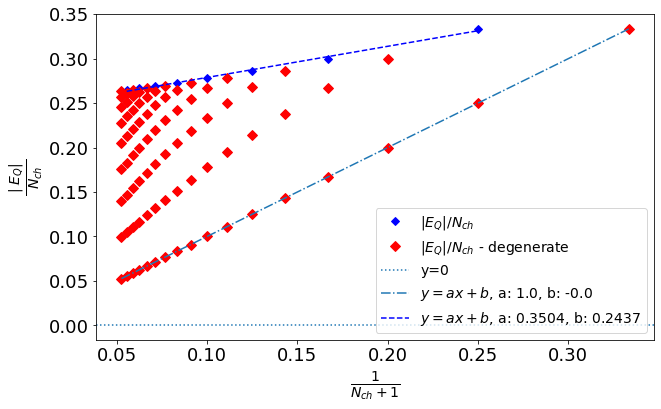
\includegraphics[width=0.7\textwidth]{QuantumEnergyperchannel}
\caption{This shows the variation of quantum energy per channel with $1/N$, where $N=N_{ch}+1$ is the total number of spins in the systems including the impurity spins.}
\label{fig:quantum_energy}
\end{figure}

\subsection{Measure of quantum fluctuations}
Here we are interested in calculating the quantum fluctuation present in the  ground state by measuring the expectation value of the spin-flip part of the Hamiltonian: ${\mathcal{Q}}\equiv \langle \psi_g | (J^x)^2+(J^y)^2 |\psi_g\rangle = \langle \psi_g | J^2 - (J^z)^2 |\psi_g\rangle$. For a general spin-$S_d$ impurity, the ground state is characterised by $J=|K/2-S_d|$, which gives $J^2=J(J+1)=(|K/2-S_d|)(|K/2-S_d|+1)$. We define $\Delta=(K/2-S_d)$ to quantify the deviation from exact screening; $\Delta=0$ represents the exactly screened problem, and $\Delta>0$ and $\Delta<0$ represents the over-screened and under-screened problems respectively. Among the degenerate ground state, the maximum quantum fluctuation will occur in the state with minimum \(|J^z|\). Since \(J\) can actually be written as \(J = |\Delta|\), \(J\) will take integer values when \(\Delta\) is integer, and the minimum value of \(|J^z|\) is then zero. Otherwise, when \(\Delta\) is half-integer, \(J\) will also take half-integer values, and the minimum value of \(|J^z|\) is \(1/2\). With these considerations, the minimum value of the quantum fluctuation, {\it per channel}, is
\begin{eqnarray}
\fl q_K = \frac{1}{K}\sqrt{Q_\text{max}} = \frac{1}{K}\sqrt{\langle \psi_g | J^2 - |J^z|_{min}^2 |\psi_g\rangle} = \begin{cases}
	\frac{1}{K}\sqrt{(|K/2-S_d|)(|K/2-S_d|+1)-1/4}, & \text{ where }\Delta\text{ is half-integer}\\
	\frac{1}{K}\sqrt{(|K/2-S_d|)(|K/2-S_d|+1)}, & \text{ where }\Delta\text{ is integer}
\end{cases}~.\quad
\end{eqnarray}
This expression is symmetric under the transformation \(\Delta \to -\Delta\), and represents a duality between the over-screened and under-screened models. In the limit of large channel number \(K\), \(q_K\) simplifies to $\lim_{K\rightarrow \infty} q_K= \lim_{K \to \infty}\frac{1}{2K}|\Delta(K)|$. Only the over- and under-screened models have non-vanishing (and equal) values of \(q_K\).


\subsection{Staggered magnetization of the star graph}
 Another probe to study the screening as a function of \(K\) is the staggered magnetization \(\vec{M}_s=\vec{S}-\vec{S}_d\). One can rewrite the Hamiltonian as $\vec{S}_d\cdot\vec{S}= \frac{1}{4}[J^2 - M_s^2]$. Since \(J\) and \(M_s\) commute with each other and hence also with the Hamiltonian, the eigenvalues of $\vec{J}^2$ and \(M_s^2\) act as good quantum numbers for in the ground states of the star graph model. The larger the value of \(\left<M_s^2\right>\), the stronger is the screening in that ground state. For single-channel case with $K=1$, the ground state is a unique 2-spin singlet $|\psi_g\rangle =\frac{1}{\sqrt{2}} (|\uparrow\downarrow\rangle-|\downarrow\uparrow\rangle = |J=0,J_z=0\rangle$, and the staggered magnetization per direction is \(M_s^2/3 = 1\), which shows the perfect screening.

Calculating the staggered magnetization for a general multichannel problem with \(K\) channels and a spin-\(S_d\) impurity reveals the breakdown of screening brought about by the presence of multiple channels. We find, in general, that the square of the staggered magnetization per channel is
\begin{eqnarray}
	\fl m_s^2 = \left< \left(\frac{1}{K}M_S\right)^2\right> = \frac{1}{K^2}\langle \psi_g | (\vec{S}_d - \vec{S})^2 |\psi_g\rangle = \frac{1}{K^2}\langle \psi_g | 2(\vec{S}_d^2 + \vec{S}^2)-\vec{J}^2 |\psi_g\rangle = \frac{2S_d(S_d+1)}{K^2}+\frac{1}{4}+\frac{1}{K}+\frac{1}{4K^2}~.
\end{eqnarray}

\begin{figure}
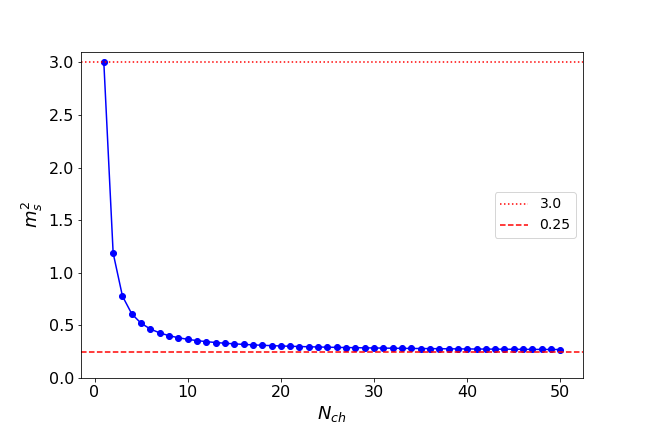
\includegraphics[width=0.7\textwidth]{Staggeredmag50.png}
\caption{This shows how the staggered magnetization changes with the number of channels $N_{ch}$.}
\label{fig:st_mag}
\end{figure}
This shows that as the number of channels increases, the value of \(m_s^2\) decreases from the perfectly-screened value of 3. For \(K \to \infty\) and keeping \(S_d\) finite, \(m_s^2\) approaches a lowered value of \(1/4\).

Due to the $SU(2)$ symmetry of the problem, the staggered magnetisation is the same along each of the three directions, such that the total value \(m_s^2\) is three times the value in any particular direction:
\begin{eqnarray}
\langle(m_s^x)^2\rangle=\langle(m_s^y)^2\rangle=\langle(m_s^z)^2\rangle=\frac{1}{3}m_s^2~,
\end{eqnarray}
As mentioned above, the single channel case displays a value of $\langle (m_s^z)^2 \rangle =1$, showing the perfect screening. If one takes the limit of \(K \to \infty\) keeping \(S_d = K/2\), we get the staggered magnetisation at exact-screening and large \(K\), and the value is $\langle (m_s^z)^2 \rangle =1/4$. This is reduced from the value at \(K=1\). This reduced value however is still greater than the value of \(1/12\) reached as \(K\to \infty\) away from exact-screening by keeping \(S_d\) finite. These conclusions can be easily understood from fig.\ref{fig:st_mag} where we have shown the variation of \(\left<m_s^2 \right>\) as a function of \(K\), keeping \(S_d=1/2\).


\subsection{Thermodynamic quantities}

\subsubsection{Impurity magnetization in terms of parity operators}
Just like the complete string operator \(\pi^z\), the modified string operator \(\sigma_d^z \pi^z\) is also a Wilson loop operator that wraps around only the outer nodes of the star graph:
\begin{eqnarray}
	\pi^z_c \equiv \sigma_d^z \pi^z = \exp\left[i \frac{\pi}{2} \left(\sum_{l=1}^K \sigma^z_l - K\right)\right] ~.
\end{eqnarray}
The expectation value of the impurity magnetization along a particular direction and in specific ground states can be related to the 't Hooft operator. We will work in the state comprised of two adjacent eigenstates of \(J^z\):
\begin{eqnarray}
	\ket{g^\theta_{J^z}} \equiv \frac{1}{\sqrt 2}\left( \ket{J^z} + e^{i\theta}\ket{J^z+1}\right), && J^z < \frac{1}{2}\left( K-1 \right)~.
\end{eqnarray}
The expectation value of the impurity magnetization operator \(\sigma_d^x\) can be expressed as
\begin{eqnarray}
	\left<\sigma_d^x\right> \equiv \langle g^\theta_{J^z} \vert \sigma_d^x \vert g^\theta_{J^z}\rangle = - \langle J^z + 1 \vert \pi^x_c \vert -J^z \rangle + \text{h.c.}~.
\end{eqnarray}
This expression relates the observable impurity magnetization to the topological 't Hooft operator \cite{Maric2020}. Evaluating the matrix elements gives
\begin{eqnarray}
	\label{sigmax}
	\left<\sigma_d^x\right> = - \frac{\sqrt{K^2 - (2J^z + 1)^2}}{2(1+K)}\cos \theta~.
\end{eqnarray}
Performing a similar calculation reveals that the impurity magnetizations along \(y\) and \(z\) in the same state are given by
\begin{eqnarray}
	\label{sigmayz}
	\left<\sigma_d^y\right> = - \frac{\sqrt{K^2 - (2J^z + 1)^2}}{2(1+K)}\sin \theta, &&\left<\sigma_d^z\right> = - \frac{2J^z + 1}{(1+K)}~.
\end{eqnarray}
Combining eqs.~\ref{sigmax} and \ref{sigmayz}, we find
\begin{eqnarray}
	\cos^2\theta\left(\left<\sigma^x_d\right>\right)^2 + \sin^2\theta\left(\left<\sigma^y_d\right>\right)^2 + \frac{1}{4}\left(\left<\sigma^z_d\right>\right)^2 = \frac{1}{4}\left(\frac{K}{1+K}\right)^2~.
\end{eqnarray}
This relation \textit{constrains the values of the magnetization} in all the directions: the \(x\) and \(y\) magnetization values have already been shown to be related to the `t Hooft operators \(\pi^x\) and \(\pi^y\) and the magnetization along \(z\) is therefore constrained in terms of the `t Hooft operators and the quantized function on the right-hand side (the function is quantized because \(K\) can only take integer values).

\subsubsection{Thermal entropy}
The star graph model can be solved to obtain the partition function, and this then allows the computation of the Helmholtz free energy and hence the thermal entropy:
\begin{eqnarray}
\fl \mathcal{F}= -k_B T\log Z, ~ ~ ~ S = -\frac{\partial \mathcal{F}}{\partial T} = -k_B \log Z -k_B T \frac{1}{Z} \frac{dZ}{dT} = -k_B \log \sum_{\epsilon} d(\epsilon) e^{-\beta \epsilon}  -\frac{1}{\beta} \frac{k_B\sum_\epsilon \epsilon d(\epsilon) e^{-\beta \epsilon} \beta^2   }{\sum_\epsilon  d(\epsilon)e^{-\beta \epsilon}}~,
\end{eqnarray}
where \(d(\epsilon)\) is the degeneracy of the state at energy \(\epsilon\). The high and low-temperature limits take very simple forms:
\begin{eqnarray}
\lim_{\beta\rightarrow \infty} S = -k_B \log_2 d(\epsilon_{G})~,\quad\lim_{\beta\rightarrow 0} S = -k_B \log \sum_\epsilon d(\epsilon)~.
\end{eqnarray}

In fig.\ref{fig:thermal_entropy}, we plot the thermal entropy (in units of $k_B \log 2$) for a range of temperatures and for different values of \(K\). At large temperatures, \(S\) saturates to integer multiples of \(k_B \log 2\), while at low-temperatures, that is not always the case. This is because the total Hilbert space dimension \(\sum _\epsilon d(\epsilon)\) is simply \(2^N\) (\(N\) being the total number of 1-particle states in the Hilbert space), and therefore \(\log \sum _\epsilon d(\epsilon) = N \log 2\) is always an integer multiple of \(N\). On the other hand, the ground state degeneracy \(d(\epsilon_G)\) is \(|K - 2 S_d|\) which is not necessarily of the form \(2^N\) and hence does not always lead to an integer multiple of \(\log 2\).

\begin{figure}
\centering
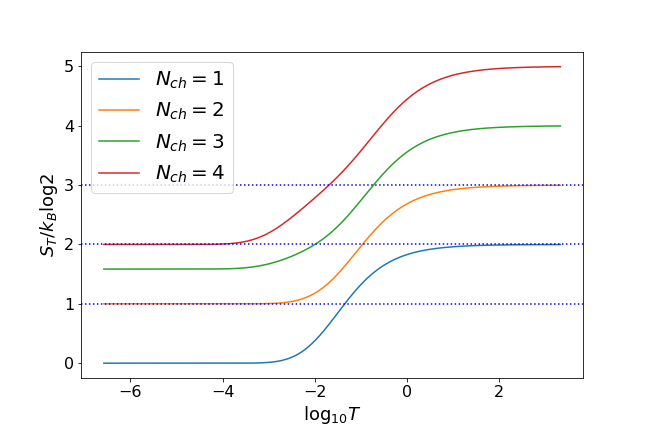
\includegraphics[width=0.7\textwidth]{ThermalEntanglementVSLogTemperature}
\caption{This shows the variation of thermal entropy with the temperature.}
\label{fig:thermal_entropy}
\end{figure}

\section{Additional Topological Features of the Local Mott liquid}
\subsection{Non-local twist operators and ground state degeneracy}

The all-to-all Hamiltonian obtained by resolving the impurity-bath quantum fluctuations is written in terms of the spinor spin operators which are individually made out of two electronic degrees of freedom.
\begin{eqnarray}
H_{eff} 
 =\frac{\beta_{\uparrow}({\mathcal{J}},\omega_{\uparrow})}{4} (S^+S^-+S^-S^+)~,
\label{eq:all-to-all_1}
\end{eqnarray}
where \(\beta_{\uparrow} ({\mathcal{J}},\omega_{\uparrow})= ({\mathcal{J}}^2 \Gamma_{\uparrow})/2, ~ ~\Gamma_{\uparrow}=(\omega_{\uparrow}-{\mathcal{J}}(S_d^z-1))^{-1}\). This spin operator is defined as $\vec{S}_i=\frac{\hbar}{2} \displaystyle\sum_{\substack{ \alpha,\beta\in \{\uparrow,\downarrow\}}}  c_{0\alpha}^{(i)\dagger} \vec{\sigma}_{\alpha\beta} c_{0\beta}^{(i)}$. In the above eq.\eqref{eq:all-to-all_1} we see the $U(1)$ symmetry of the effective Hamiltonian. Using the spinor representation, we obtain the spin creation operation in terms of the electronic degree of freedom:
\begin{eqnarray}
S_i^+ = \frac{\hbar}{2} \displaystyle\sum_{\alpha,\beta\in \{\uparrow\downarrow\}} c_{0\alpha}^{(i)\dagger} {\sigma}^{+}_{\alpha\beta} c_{0\beta}^{(i)}
=\frac{\hbar}{2} c_{0\uparrow}^{(i)\dagger} c_{0\downarrow}^{(i)}, \quad S_i^z &= \frac{\hbar}{2} \displaystyle\sum_{\alpha,\beta\in \{\uparrow\downarrow\}} c_{0\alpha}^{(i)\dagger} {\sigma}^{z}_{\alpha\beta} c_{0\beta}^{(i)} \nonumber\\
									       &=\frac{\hbar}{2} (c_{0\uparrow}^{(i)\dagger} c_{0\uparrow}^{(i)} - c_{0\downarrow}^{(i)\dagger} c_{0\downarrow}^{(i)} )~.
\end{eqnarray}
This spinor is simply the Anderson pseudo-spin formulation in the spin channel. The spin-creation operator ($S_i^+$) involves the simultaneous creation of an electron-hole pair at the real space origin of the $i^{th}$ conduction channel. The condensation of such electron-hole pairs has already been shown in ~\cite{anirbanmott1,anirbanmott2}. Thus, for this effective Hamiltonian, one can define twist-translation operations to construct the gauge theory and unveil any hidden degeneracy.

Let's recall the effective Hamiltonian
\begin{eqnarray}
H_{eff} &=& \frac{\beta_{\uparrow}(\alpha,\omega_{\uparrow})}{4} \left[ \displaystyle\sum_{ij} S_i^+S_j^- ~+ \textrm{h.c.} \right]~,
\end{eqnarray}
where $i,j$ are the channel indices. Due to the all-to-all nature of the connectivity, one can draw a total of $K!$ possible unique closed paths ($\mathcal{C}_{\mu}$) such that each node (channel) is touched exactly once. These curves lead to $K!$ translation operators ($\hat{T}_{\mu}$) which keeps the Hamiltonian invariant. Let's define one such translation operator $\hat{T}_{\mu}=e^{i\hat{P}^{cm}_{{\mu}}}$ which gives a periodic shift along the closed path $\mathcal{C}_{\mu}$. The twist operator along the path $\mathcal{C}_{\mu}$ is given by
\begin{eqnarray}
\hat{\mathcal{O}}_{\mu} &=& \exp({i\frac{2\pi}{K} \displaystyle\sum_{\substack{j=1\\ \mathcal{C}_{\mu}}}^{K} j S_j^z} )~,
\end{eqnarray}
The action of the translation operator on \(S_j^z\) is to translate it by one channel index: $\hat{T}_{\mu} S_j^z \hat T^\dagger_\mu = S_{j+1}^z$ where $j+1$ and $j$ are the nearest neighbor on the closed path $\mathcal{C}_{\mu}$. Then the braiding rule between the twist and translation operators are give as
\begin{eqnarray}
\hat{T}_{\mu}\hat{\mathcal{O}}_{\mu} \hat{T}^{\dagger}_{\mu} \hat{\mathcal{O}}_{\mu}^{\dagger} = \exp\{i[2\pi S_1^z-\frac{2\pi}{K}S^z]\} = \exp\{i[\pm \pi - \frac{2\pi}{K} S^z]\} =\exp(i\frac{2\pi p}{q})~.
\end{eqnarray}
The availability of the non-trivial braiding statistics between these twist and translation operators is possible if $p\neq 0$ and $q\neq \infty$. Further simplification leads to the condition
\begin{eqnarray}
 \pm\pi -\frac{2\pi}{K} S^z = \frac{2\pi p}{q} \implies  \pm\frac{1}{2}-\frac{S^z}{K} = \frac{p}{q} , ~ ~ ~ \frac{(\pm K-2S^z)}{2K} = \frac{p}{q}~,
\end{eqnarray} 
where $p,q$ are mutual primes. We know that the $S^z$ can take values $(\mp K/2\pm m)$ where $m$ is a integer $0 \leq m \leq K$. Putting this value in the above equation leads to two possible solutions.
\begin{eqnarray}
\frac{(K-m)}{K} &=& \frac{p}{q} ~,\quad \frac{-m}{K}=\frac{p}{q}~.
\end{eqnarray}
For the first case where $K-m=p$, we can see that $m=K$ makes $p$ trivial, and hence the allowed values are $m=0,\cdots,K-1$, which represents the corresponding $S^z$ eigenvalues 
\begin{eqnarray}
&&-K/2,-K/2+1,\cdots,K/2-2,K/2-1~.
\end{eqnarray}
Similarly the second case implies, $-m=p$, but $p=0$ is not allowed as this makes the braiding statistics trivial, thus the possible $S^z$ values are 
\begin{eqnarray}
-K/2+1,-K/2+2,\cdots,K/2-1,K/2~.
\end{eqnarray}
This gives the general braiding statistics between the twist and the translation,
\begin{eqnarray}
\hat{T}_{\mu}\hat{\mathcal{O}_{\mu}} \hat{T}^{\dagger}_{\mu}\hat{\mathcal{O}_{\mu}}^{\dagger} &=& e^{i\frac{2\pi p}{K}}~,
\end{eqnarray}
where $p$ corresponds to different $S^z$ states, related as $p=\pm K/2-S^z$. Thus we can see that there are $K$ possible $S^z$ plateau states in the all-to-all model where each plateau is $K$ fold degenerate. This $p/K$ is similar to the filling factor of the fractional quantum Hall effect. There are $K!$ pairs of twist and translation operators corresponding to different closed paths $\mathcal{C}_{\mu}$ which can probe this degeneracy.

\subsection{Action on the Hamiltonian}
We will now obtain the action of these twist operators on the Hamiltonian in eq.~\ref{eq:all-to-all_1}. Due to the all-to-all nature of the effective Hamiltonian one can find $K!$ possible relative arrangement of those $K$ channels which keeps the Hamiltonian invariant. Here we briefly discuss the choice of the closed-loop $\mathcal{C}_{\mu}$ and the insertion of the flux. As shown in the Fig.\ref{fig:stargraph-to-alltoall}(b) we have chosen a particular closed path which crosses all the outer spin only once. We embed that closed-loop on a plane and put the flux perpendicular to the plane through the closed loop. One can find a different closed loop where the ordering of the outer spins will be different. The action of the translation operator shifts the outer spins along this closed curve by one step.

\begin{figure}[htpb]
	\centering
	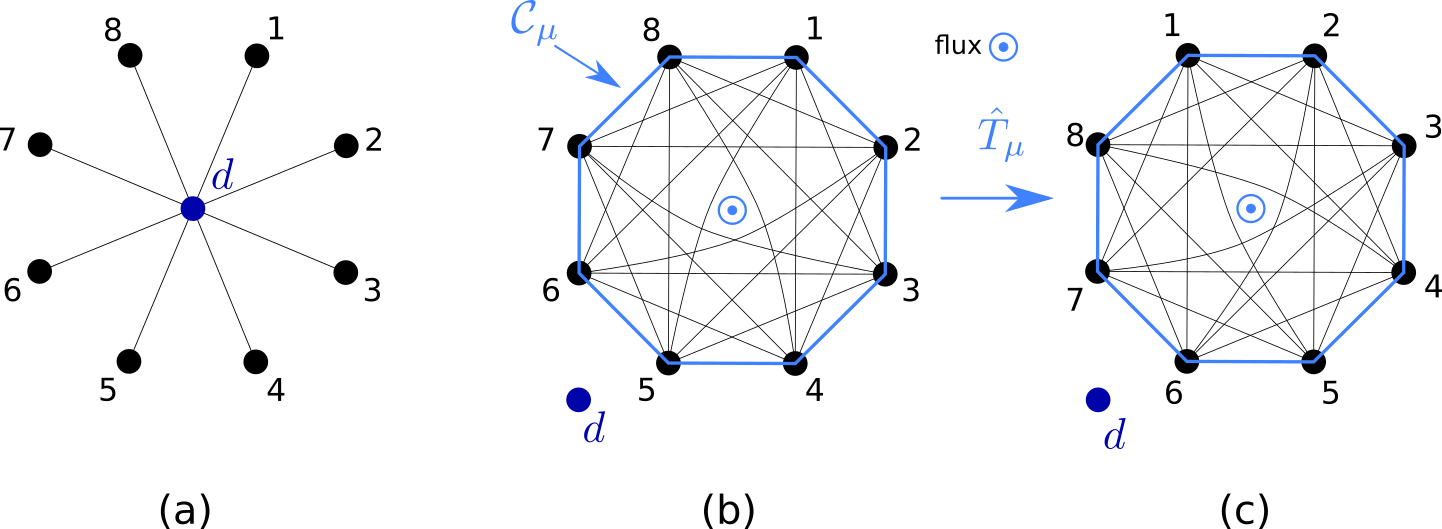
\includegraphics[width=0.8\textwidth]{stargraphtoalltoall.png}
	\caption{(a) Schematic diagram of $8-$channel multichannel Kondo model zero mode in zero bandwidth limit. (b) All-to-all model obtained by disentangling the impurity spin from the bath zero modes. $C_{\mu}$ is a particular closed curve. (c) Translated configuration along the curve $C_{\mu}$ by one unit.}
	\label{fig:stargraph-to-alltoall}
\end{figure}

The action of the twist operator on the $S^x$ is determined in the following calculation
\begin{eqnarray}
\hat{O}_{\mu} S^x \hat{O}^{\dagger}_{\mu} = \exp({i\frac{2\pi}{K} \displaystyle\sum_{\substack{j=1\\ \mathcal{P}_{\mu}}}^{K} j S_j^z} )S^x \exp({-i\frac{2\pi}{K} \displaystyle\sum_{\substack{j=1\\ \mathcal{P}_{\mu}}}^{K} j S_j^z} ) = e^{X} S^x e^{-X}~.
\end{eqnarray}
To simplify the calculation, we define $i\frac{2\pi}{K}=\Omega$, thus $X=\Omega\sum_j jS^z_j$. Thus we get
\begin{eqnarray}
e^X S^x e^{-X}= S^x+[X,S^x] + \frac{1}{2!}[X,[X,S^x]] +\cdots = \sum_l ( S^x_l \cos \theta_l -  S_l^y \sin \theta_l ) ~,\nonumber\\
e^X S^y e^{-X}= \sum_l  (S^y_l \cos\theta_l  + S^x_l \sin\theta_l)\nonumber\\
\theta_l=\frac{2\pi l}{K}~.
\end{eqnarray}
As already defined, $\theta_l=\frac{2\pi l}{K}=\frac{2\pi (K-n)}{K}$, where $n$ is an integer. We can see that in the large channel limit $\theta_l $ becomes inter multiple of $2\pi$. Thus in the large channel limit
\begin{eqnarray}
	\hspace*{-20pt}\lim_{K\rightarrow \infty}\hat{\mathcal{O}}_{\mu} H_{eff} \hat{\mathcal{O}}_{\mu}^{\dagger}\nonumber = \frac{\beta_{\uparrow}(\alpha,\omega_{\uparrow})}{2} \left[ \hat{\mathcal{O}}_{\mu} S^x \hat{\mathcal{O}}_{\mu}^{\dagger} \hat{\mathcal{O}}_{\mu} S^x \hat{\mathcal{O}}_{\mu}^{\dagger}  + \hat{\mathcal{O}}_{\mu} S^y \hat{\mathcal{O}}_{\mu}^{\dagger} \hat{\mathcal{O}}_{\mu} S^y \hat{\mathcal{O}}_{\mu}^{\dagger}  \right] = \frac{\beta_{\uparrow}(\alpha,\omega_{\uparrow})}{2} \left[  S^{x2}+S^{y2}  \right] = H_{eff},\\
\hspace*{-20pt} \lim_{K\rightarrow \infty } [\hat{\mathcal{O}},H_{eff}] = 0~.
\label{eq:hamiltonian_twisted}
\end{eqnarray}
 
Since the translation operator $\hat{T}_{\mu}=e^{i\hat{\mathcal{P}}_{\mu}}$ commutes with the Hamiltonian, so does the generator $\hat{\mathcal{P}}_{\mu}$. We can label the $j^{th}$ state with the eigenvalues of this operator $\hat{\mathcal{P}_{\mu}}$ as $|p^{j}_{\mu}\rangle$. The action of these twist and translation operators on these states are
\begin{eqnarray}
\hspace*{-20pt}\hat{T}_{\mu} |p^j_{\mu} \rangle = e^{i\hat{\mathcal{P}}_{\mu}} |p^j_{\mu} \rangle = e^{ip^j_{\mu}} |p^j_{\mu}\rangle, ~ ~ ~ ~ \hat{T}_{\mu} \hat{\mathcal{O}}_{\mu} |p^j_{\mu} \rangle =  \hat{\mathcal{O}}_{\mu} \hat{T}_{\mu} e^{i\frac{2\pi m}{K}} |p^j_{\mu}\rangle = \hat{\mathcal{O}}_{\mu}   e^{i(\frac{2\pi m}{K}+p_{\mu}^j)} |p^j_{\mu}\rangle~,\quad\frac{2\pi m}{K} \equiv p_{\mu}^{m}~, \nonumber\\
\hspace*{-20pt}\hat{T}_{\mu} \left( \hat{\mathcal{O}}_{\mu} |p^j_{\mu} \rangle  \right) = e^{i(p_{\mu}^{m}+p_{\mu}^j)} \left( \hat{\mathcal{O}}_{\mu}    |p^j_{\mu}\rangle \right)~,
\end{eqnarray}
where $m$ represents different $S^z$ plateaux. This shows that  $\hat{\mathcal{O}}_{\mu} |p^j_{\mu} \rangle $ is again an eigenstate of the translation operator, but with an eigenvalue that is different from $|p^j_{\mu} \rangle $, and is thus orthogonal to $\ket{p^j_{\mu}}$. Similarly, one can in general show that $\langle p^j_{\mu} | \hat{\mathcal{O}}^{q}_{\mu} |p^j_{\mu} \rangle=0$, where $q$ is any integer. Also in the large $K$ limit we can see from the eq.\eqref{eq:hamiltonian_twisted} that these different twisted states has same energy. Which shows that at each plateau state labeled by the $S^z$ eigenvalue has $K$ fold degenerate eigenstates labeled by the eigenvalue of the translation operators. The complete set of commuting observables is therefore formed by $H,S^z,\hat{T}$, and states can be labeled as  $|E,S^z_j,P^j_{\mu}\rangle$. 




\section{Effect of conduction bath excitations on the fixed point theory}
\subsection{Non-Fermi liquid signatures in momentum space for 2-channel Kondo}
Obtaining the effective Hamiltonian involves obtaining the low energy excitations on top of the ground state of the star graph. The large-energy excitations involve spin flips. This guides the separation of the Hamiltonian into a diagonal and an off-diagonal piece:
\begin{eqnarray}
	H = H_d + V = \underbrace{H_0 + J S_d^z s_\text{tot}^z}_{H_d} + \underbrace{\frac{J}{2}S_d^+ s_\text{tot}^- + \text{h.c.}}_{V + V^\dagger}
\end{eqnarray}
We define \(V\) as the interaction term that decreases \(s_\text{tot}^z\) by 1: \(V \ket{s_\text{tot}^z} \to \ket{s_\text{tot}^z - 1}\). Similarly, we define \(V^\dagger \ket{s_\text{tot}^z} \to \ket{s_\text{tot}^z + 1}\). The Schrodinger equation for the ground state can be written as
\begin{eqnarray}
	E_\text{gs}\ket{\Psi_\text{gs}} = H \ket{\Psi_\text{gs}} = \left(H_d + V\right)\ket{\Psi_\text{gs}} \nonumber\\
	\implies \left(E_\text{gs} - H_d\right)\sum C_{S_d^z, s_\text{tot},s_\text{tot}^z}\ket{S_d^z, s_\text{tot}, s_\text{tot}^z} = V\sum C_{S_d^z, s_\text{tot},s_\text{tot}^z}\ket{S_d^z, s_\text{tot}, s_\text{tot}^z}
\end{eqnarray}
\(E_\text{gs}\) is the ground state energy, and can be replaced by the star graph ground state energy if we remove the kinetic energy cost via normal ordering: \(E_\text{gs} = -\frac{J}{2}\left(\frac{K}{2}+1\right) \). Since the interaction part \(V\) only changes \(S_d^z \to -S_d^z\) and \(s^z_\text{tot} \to s^z_\text{tot} \pm 1\), we can simplify the equation into individual smaller equations. For the state \((s_\text{tot},s^z_\text{tot}) = (1,0)\), equations are
\begin{eqnarray}
	\label{eff_ham_Sdz_10}
	\hspace*{-30pt}E_\text{gs} \ket{\frac{1}{2}, 1, 0} = \left(H_d + V \frac{1}{E_\text{gs} - H_d}V^\dagger\right) \ket{\frac{1}{2}, 1, 0}, \quad E_\text{gs} \ket{-\frac{1}{2}, 1, 0} = \left(H_d + V^\dagger \frac{1}{E_\text{gs} - H_d} V\right) \ket{-\frac{1}{2}, 1, 0}~.
\end{eqnarray}
These represent the Schrodinger equation for the states \(\ket{S_d^z, 1, 0}\), and the right hand sides therefore give the effective Hamiltonians for those states. If we combine the states into a single subspace \(\ket{1,0}= \left\{\ket{\frac{1}{2}, 1, 0}, \ket{-\frac{1}{2}, 1, 0}\right\}\), the effective Hamiltonian for this composite subspace becomes the sum of the two parts:
\begin{eqnarray}
	\label{eff_ham_10}
	H^{1,0}_\text{eff}\ket{1, 0}\bra{1, 0} = \left(H_d + V G_0 V^\dagger + V^\dagger G_0  V\right) \ket{1, 0}~,
\end{eqnarray}
where \(G_0 = \left(E_\text{gs} - H_d\right)^{-1}\). To calculate these effective Hamiltonians, we will expand the denominator in powers of in \(H_0^n/J^{n+1}, n=0,1,2,\ldots\). Expanding up to \(n=2\) and keeping at most two particle interaction terms, 
the effective Hamiltonian is
\begin{eqnarray}
	H_\text{eff}^{1, 0} = H_0 + \frac{J^2}{2\left(E_\text{gs} + \frac{J}{2}\right)}&\left[1 + \frac{ H_0 + \left(\frac{1}{2} + S_d^z\right) s^+_\text{tot}X_{1,\text{tot}} - \left(\frac{1}{2} - S_d^z\right) s^-_\text{tot}X^\dagger_{1,\text{tot}}}{2 \left(E_\text{gs} + \frac{J}{2}\right)} + \frac{H_0^2}{\left(E_\text{gs} + \frac{J}{2}\right)^2} \right.\nonumber\\
&\left.- \frac{Z_{1,\text{tot}} H_0}{\left(E_\text{gs} + \frac{J}{2}\right)^3} \right]~.
\end{eqnarray}
We employed the definitions 
\begin{eqnarray}
X_{n,\text{tot}} \equiv  \sum_l \sum_{k,k^\prime}\left(\epsilon_k - \epsilon_{k^\prime}\right)^n c^\dagger_{k \downarrow}c_{k^\prime \uparrow}, ~ ~ ~ Z_{1,\text{tot}} \equiv \sum_{k,k^\prime,l}\left( \epsilon_k - \epsilon_{k^\prime} \right) \frac{1}{2}\left(c^\dagger_{k \uparrow,l}c_{k^\prime \uparrow,l} - c^\dagger_{k \downarrow,l}c_{k^\prime \downarrow,l}\right)~.
\end{eqnarray}
There are several non-Fermi liquid terms of the form \(s^+_\text{tot}X_{1,\text{tot}}, s^-_\text{tot}X^\dagger_{1,\text{tot}},Z_{1,\text{tot}} H_0\). These arise because of the degenerate manifold and the increased availability of states in the Hilbert space for scattering, as compared to the unique singlet ground state of the single-channel Kondo model.


\subsection{Low-temperature thermodynamic behaviour}
The non-Fermi liquid (NFL) nature of the effective Hamiltonian can be demonstrated through a calculation of certain thermodynamic quantities like the impurity specific heat and the magnetic susceptibility. We begin by calculating the self-energy of this NFL hamiltonian. In real space, one can extract a diagonal piece from the effective Hamiltonian by using the fermionic anticommutation relations.
\begin{eqnarray}
H_{eff}^{off,(2)} |_{diag} &=& -(16t^2/3) [ (S_1^z)^2+ (S_2^z)^2 ] ~,
\end{eqnarray}
the corresponding momentum space Hamiltonian is obtained from the Fourier transform:
\begin{eqnarray}
H_{eff}^{off,(2)} |_{diag}= -\frac{4t^2}{3} \frac{1}{N} \left[ \displaystyle\sum_{k,\sigma} n_{k\sigma}(1-\frac{1}{N} \displaystyle\sum_{k_2}  n_{k_2,-\sigma}  ) + \displaystyle\sum_{k,\sigma} \tilde{n}_{k\sigma} ( 1-\frac{1}{N} \displaystyle\sum_{ k_2} \tilde{n}_{k_2,-\sigma}  ) \right]~.
\end{eqnarray}
The above relation leads to the self-energy correction to the kinetic energy, which is
\begin{eqnarray}
\bar{\epsilon} _k-\epsilon_k = \Sigma_k = -\frac{4t^2}{3N^2}\left(1-\frac{N}{e^{(\epsilon_k-\mu)/k_BT}+1}\right)~.
\label{eq:self-energy-NFL}
\end{eqnarray}
Using the self-energy we calculate the impurity specific heat defined as $C_{imp}=C(J^*)-C(0)$ which is defined as
\begin{eqnarray}
C_{imp} &=& \sum_{\Lambda,\sigma} \beta \left[ \frac{(\bar{\epsilon}_{\Lambda})^2 e^{\beta \bar{\epsilon}_{\Lambda}}}{( e^{\beta \bar{\epsilon}_{\Lambda}} +1)^2}  -\frac{({\epsilon}_{\Lambda})^2 e^{\beta {\epsilon}_{\Lambda}}}{( e^{\beta {\epsilon}_{\Lambda}} +1)^2} \right]~.
\end{eqnarray}
\begin{figure}[!htb]
\centering
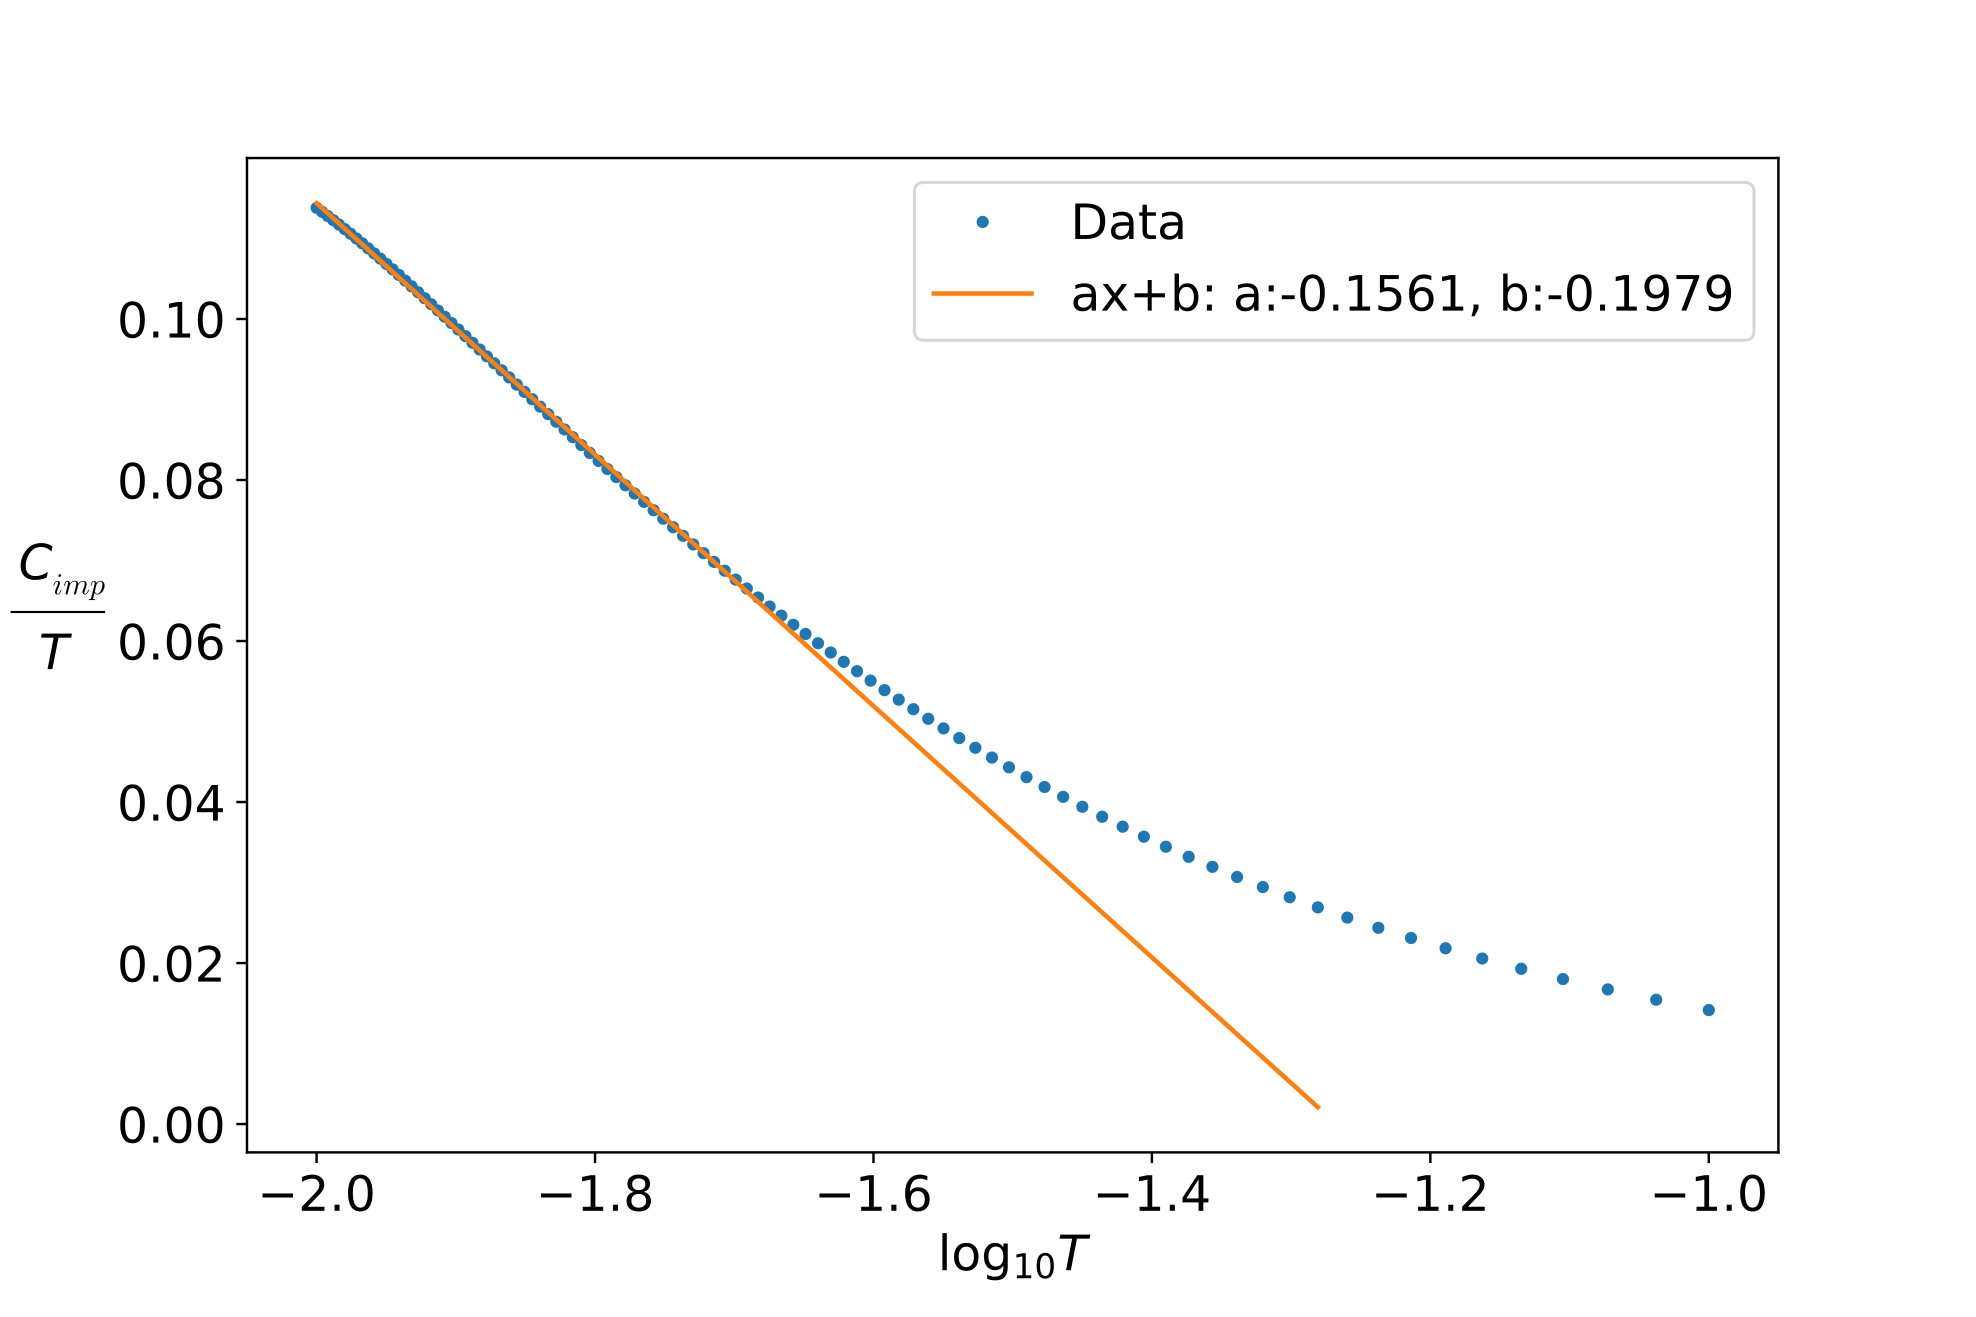
\includegraphics[width=0.49\textwidth]{FINALfittedCvt0p1.png}
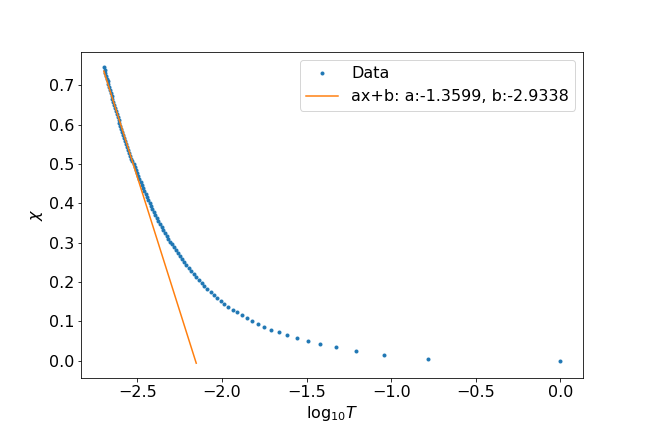
\includegraphics[width=0.49\textwidth]{NFLChilog0p1}
\caption{Anomalous contribution to the impurity specfic heat (left) and the maginetic susceptibility (right) arising from the non-Fermi liquid component}
\label{fig:Cv_imp}
\end{figure}
Using the self-energy obtained above, we extract the low-temperature behaviour of the impurity specific heat in the two-channel model for $t=0.1$ and $\mathcal{J}=1$, and it is shown in the left panel of fig.~\ref{fig:Cv_imp}. We find that at low-temperatures, the Sommerfeld coefficient \(C_\text{imp}/T\) follows a logarithmic behaviour for the two-channel case, which is in agreement with the results known in the literature~\cite{affleck_1991_overscreen,affleck_ludwig_1991,affleck_pang_cox_1992,affleck1993exact,
parcollet_olivier_large_N,affleck_2005,emery_kivelson,clarke_giamarchi_1993,zarand_2000,
vondelft_prl_1998,schofield_1997,bullaNRGreview,affleck_pang_cox_1992,pang_cox_1991,
andrei_destri_1984,Tsvelick1984,Tsvelick_1985,andrei_jerez_1995,zarand_costi_2002,
sengupta_1994,fabrizio_nozieres_1995,Coleman_tsvelik,fabrizio_gogolin_1995}.
\begin{eqnarray}
\frac{C_{imp}}{T} \propto \log T~.
\end{eqnarray}
To calculate the magnetic susceptibility, we numerically diagonalise the low-energy effective Hamiltonian, and use the following expression:
\begin{eqnarray}
\chi &=& \beta\left[\frac{\sum e^{-\beta \bar{\epsilon}_{\Lambda}} \langle \bar{S}^{z2} \rangle}{\sum e^{-\beta \bar{\epsilon}_{\Lambda}} } -\frac{\sum e^{-\beta \epsilon_{\Lambda}} \langle S^{z2 }\rangle }{\sum e^{-\beta \epsilon_{\Lambda}} } \right] ~.
\end{eqnarray}
The result is shown in the right panel of fig.~\ref{fig:Cv_imp}, and we find that at low temperatures, the susceptibility has a logarithmic behaviour.
\begin{eqnarray}
\chi(T) &\propto& \log T
\end{eqnarray}

We also calculated the Wilson ratio $C_{imp}/T\chi$, and we find that taking up to three sites on each conduction channel leads to a value of $ W = 8.3$, which is greater than the known value of \(8/3\)~\cite{affleck_1991_overscreen,affleck_ludwig_1991,affleck_pang_cox_1992,affleck1993exact,
parcollet_olivier_large_N,affleck_2005,emery_kivelson,clarke_giamarchi_1993,zarand_2000,
vondelft_prl_1998,schofield_1997,bullaNRGreview,affleck_pang_cox_1992,pang_cox_1991,
andrei_destri_1984,Tsvelick1984,Tsvelick_1985,andrei_jerez_1995,zarand_costi_2002,
sengupta_1994,fabrizio_nozieres_1995,Coleman_tsvelik,fabrizio_gogolin_1995}. We find that taking less number of sites leads to a yet higher value of \(W\), which shows that taking more number of sites will lead to a value of \(W\) that is lower than \(8.3\) and closer to \(8/3\). 

\subsection{Orthogonality catastrophe in the gapless excitations of the 2CK}
By combining the ground-states of the star graph and the effect of hopping into the remaining lattice, it is possible to demonstrate an orthogonality catastrophe~\cite{anderson1967infrared,varma2002singular} in the new modified ground-state. The full Hilbert space consists of the star graph (formed by the impurity site and the zeroth sites of all channels) and the {\it reduced} conduction bath (formed by sites 1 and beyond in all channels). All terms in the Hamiltonian conserve the total spin \(S_\text{tot}^z = S_d^z + S_0^z + s^z\) composed of the impurity spin \(S_d^z\), the zeroth site spin \(S_0^z = \sum_l S_{0,(l)}^z\) and the spin of the reduced bath \(s^z\). We will work in the \(S_\text{tot}^z = 0\) sector. To construct the non-magnetic ground-states, we will assume the presence of gapless excitations vanishingly close to the Fermi surface in the reduced conduction bath. If \(\ket{\phi}\) represents the filled Fermi volume configuration of all the channels, these excitations can be written as \(\ket{e_\sigma^{(l)}} \equiv e^\dagger_{\sigma,(l)} \ket{\phi} = \sum_{k \in \text{FS}}c^\dagger_{k\sigma,(l)} \ket{\phi}\), where \(l \in \left\{1,2\right\} \) is the channel index. Apart from these states, we have the star graph ground-states at \(S_\text{sg}^z \equiv S_d^z + S_0^z = \pm \frac{1}{2}\): \(\ket{S_\text{sg}^z = \frac{\sigma}{2}} = \frac{1}{\sqrt 6}\left( \ket{\sigma,\sigma,\bar\sigma} + \ket{\sigma,\bar\sigma,\sigma} -2\ket{\bar\sigma,\sigma,\sigma} \right),~ \sigma=\pm 1 \). Within each ket, the three symbols indicate the configuration of the impurity spin, the zeroth site of the first channel and that of the second channel respectively. In the absence of any hopping between the star graph and the reduced conduction bath, the full non-magnetic ground states are then of the form:
\begin{equation}\begin{aligned}
	\ket{l,\sigma} = \ket{S^z_\text{sg}=\frac{-\sigma}{2}}\otimes\ket{e_{\sigma}^{(l)}},~l\in\left\{ 1,2 \right\},~\sigma=\pm 1~.
\end{aligned}\end{equation}
We now introduce the hopping \(H_\text{int}\) between the star graph and the reduced conduction bath,
\begin{equation}\begin{aligned}
	H_\text{int} = -t\frac{1}{\sqrt N}\sum_{k,\sigma,l}\left( c^\dagger_{k\sigma,(l)}c_{0\sigma,(l)} + \text{h.c.} \right)~,
\end{aligned}\end{equation}
and treat it under degenerate perturbation theory. Since all terms in the Hamiltonian conserve the number of particles in each channel, the states with different \(l\) do not mix. For each value of \(l\), the \(2\times 2\) matrix of \(H_\text{int}\) takes the form
\begin{equation}\begin{aligned}
	H_\text{int} = \frac{4t^2}{J^*}\begin{pmatrix} 0 & 1 \\ 1 & 0 \end{pmatrix} ~.
\end{aligned}\end{equation}
The non-zero off-diagonal terms arise because of second-order scattering processes.
Diagonalising this gives the modified new ground-states:
\begin{equation}\begin{aligned}
	\ket{\psi_\pm^{(l)}} = \frac{1}{\sqrt 2}\left(\ket{l,\uparrow} \pm \ket{l,\downarrow}\right), E_\pm = -4t^2/J^*~.
\end{aligned}\end{equation}
We can now calculate the residue for scattering processes of the kind \(e^\dagger_{\sigma,(l)} e_{\bar\sigma,(l)}\), in the new ground-state and excited state, and they are found to vanish:
\begin{equation}\begin{aligned}
	Z = |\braket{\psi_+^{(l)}| e^\dagger_{\uparrow,(l)} e_{\downarrow,(l)} | \psi_-^{(l)}}|^2 = \left|\bra{\psi_+^{(l)}}\left(\ket{S_\text{sg}^z=\frac{1}{2}}\ket{e_\uparrow^{(l)}}\right)\right|^2 = 0
\end{aligned}\end{equation}
This shows that the single-particle excitations are no longer long-lived, signaling the orthogonality catastrophe.



\subsection{Three channel LEH}
Similar to the two channel case, we here calculate the low energy effective Hamiltonian for three channel Kondo problem by introducing the real space hopping on top of the zero mode three-channel star graph model. This zero mode three channel star graph model has three fold degenerate ground states with total $2^4=16$ states in the eigenspectrum. The three degenerate ground states are given as 
\begin{eqnarray}
\fl |\alpha_{-1}\rangle = c|1000 \rangle-b (|0100 \rangle + |0010 \rangle+ | 0001 \rangle), ~ ~ |\alpha_{+1}\rangle = b(|1110 \rangle+ | 1101 \rangle + | 1011 \rangle)-c | 0111 \rangle,\nonumber\\
\fl |\alpha_0\rangle = -a(|1100 \rangle + |1010\rangle +|1001 \rangle) + a(|0110 \rangle+| 0101 \rangle +| 0011\rangle)~,
\end{eqnarray}
where $a=0.408$, $b=0.289$, $c=0.866$. Here the state is represented by $|n_{d},n_1,n_2,n_3\rangle$, where $n_i=1/0$ represents the spin configuration $S_i^z=\pm 1/2$ respectively. Next we use degenerate perturbation theory to get the LEH which contains diagonal and off-diagonal terms. In this case we get non-zero contribution from all the three ground states $|J^z=-1\rangle$, $|J^z=0\rangle$ and $|J^z=1\rangle$. We get the diagonal contribution to the LEH in the second order to be
\begin{eqnarray}
H^{(2)}_{eff, diag} &=& - \frac{7.2 J^2}{\alpha} \hat{I}~.
\end{eqnarray}
The contribution associated with different ground states $|J^z=-1\rangle$, $|J^z=0\rangle$ and $|J^z=1\rangle$ is given respectively as $- \frac{2.4 J^2}{\alpha} \hat{I} + \hat{\mathcal{F}},- \frac{2.4 J^2}{\alpha} \hat{I} ,- \frac{2.4 J^2}{\alpha} \hat{I} - \hat{\mathcal{F} }$,
where $\hat{\mathcal{F}}$ is a function of diagonal number operators of sites nearest neighbor to the zeroth site of each channels. The off-diagonal terms in the LEH is appearing due to the scattering between pair of degenerate states $(\alpha_0,\alpha_{+1})$ and $(\alpha_0,\alpha_{-1})$, there is no contribution in the second order coming from the scattering between $(\alpha_{-1},\alpha_{+1})$. The effective low energy Hamiltonian in the second order is given as
\begin{eqnarray}
	H^{(2)}_{eff,off-diag} = \sum_{\substack{(ijk)=\\(123),(231),(312)}}&\left[ c_{i\uparrow}c_{i\downarrow}^{\dagger} \left( -2ab \left\{ \Sigma_{jk} +c_{j\uparrow}^{\dagger}c_{j\downarrow}c_{k\uparrow}c_{k\downarrow}^{\downarrow} \right\} -ac(\Omega_{jk}+\tilde{\Omega}_{jk}) \right) \right.\nonumber\\
										  &\left. + \textrm{h.c.}\right] \otimes \hat{\Xi}_l~,
\end{eqnarray}
where the different operators have the following definitions:
\begin{eqnarray}
\fl \Sigma_{i,j} = n_{i\uparrow}(1-n_{i\downarrow}) (1-n_{j\uparrow})n_{j\downarrow} + (1-n_{i\uparrow})n_{i\downarrow} n_{j\uparrow} (1 -n_{j\downarrow}), ~ ~\Omega_{i,j} =4S_i^z S_j^z n_{i\uparrow} n_{j\uparrow}, ~ ~ \tilde{\Omega}_{i,j} = 4S_{i}^zS_j^z (1-n_{i\uparrow})(1-n_{j\uparrow}) \nonumber~,\\
\fl \hat{\Xi}_l=  ( c_{l_1\uparrow}^{\dagger} c_{l_1\downarrow} +c_{l_2\uparrow}^{\dagger} c_{l_2\downarrow} + c_{l_3\uparrow}^{\dagger} c_{l_3\downarrow} + \textrm{h.c.})~.
\end{eqnarray}

\section{Hamiltonian RG of spin-\(S\) impurity MCK Model}
\label{appendix_urg}

\subsection{Details of the URG method}

The non-trivial nature of the impurity problem arises from the fact that the many-particle correlation between the impurity spin and the conduction electrons induces a many-particle interaction among the conduction electron states. This means that within the conduction band, the states at high and low energies get entangled with each other, leading to what is called UV-IR mixing. One of the methods of obtaining the low-energy physics while taking into account the effect of the high energy degrees of freedom is the renormalisation group (RG) approach. The specific variant of RG used in this work is the unitary renormalisation group (URG) method developed by some of us in Refs.~\cite{santanukagome,anirbanmott1,anirbanmott2,1dhubjhep,siddharthacpi,mukherjeeMERG2022,kondo_urg}. The URG proceeds by applying unitary transformations on the Hamiltonian in order to decouple the high-energy \(k-\)states, leading to a reduction in the effective bandwidth and changes in the couplings for the low-energy degrees of freedom in the process. This leads to a sequence of renormalised Hamiltonians, and hence the coupling RG equations. While this is similar in spirit to the Poor Man's scaling approach of Anderson as applied to the single channel Kondo model~\cite{anderson1970}, there are several differences between the methods that will be apparent when we describe the method in more detail below.

We start by defining a UV-IR scheme for the single-particle electronic states \(\vec k = (k_F + |\vec k|) \hat k\). We label the single-particle \(\vec k-\)states in terms of their normal distance $\Lambda = |\vec k|$ from the Fermi surface (FS) and the orientation of the unit vectors $\hat{s} = \hat k$, where $\hat{s}=\frac{\nabla\epsilon_{\mathbf{k}}}{|\nabla\epsilon_{\mathbf{k}}|}|_{\epsilon_{\mathbf{k}}=E_{F}}$. Each \(\hat s\) represents a direction that is normal to the FS. Combining these two labels with the spin index \(\sigma=\uparrow,\downarrow\), each single-particle state can be uniquely labelled as $\ket{j,l} = \ket{(k_F + \Lambda_j) \hat s,\sigma}, l\equiv (\hat{s},\sigma)$. The $\Lambda$'s are arranged as follows: $\Lambda_{N}>\Lambda_{N-1}>\ldots>0$, such that \(\Lambda_N\) is farthest from the Fermi surface and is hence the most energetic (UV) while \(\Lambda_0\) is closest to the Fermi surface and is least energetic (IR). The URG proceeds by disentangling these states \(\Lambda_j\), starting from those near the UV and gradually scaling towards the IR. This leads to the Hamiltonian flow equation~\cite{anirbanurg1}
\begin{eqnarray}
\centering
\label{urg_map}
H_{(j-1)}=U_{(j)}H_{(j)}U^{\dagger}_{(j)}~,
\end{eqnarray}
where the unitary operation $U_{(j)}$ is the unitary map at RG step $j$. 
$U_{(j)}$ disentangles all the electronic states 
$|\mathbf{k}_{\Lambda_{j}\hat{s}_{m}},\sigma\rangle$
on the isogeometric curve and has the form~\cite{anirbanmott1,anirbanurg1}
\begin{eqnarray}
\centering U_{(j)}=\prod_{l}U_{j,l}, U_{j,l}=\frac{1}{\sqrt{2}}\sum_l [1+\eta_{j,l}-\eta^{\dagger}_{j,l}]~,
\end{eqnarray}
where \(l\) sums over the states on the isoenergetic shell at distance \(\Lambda_j\), and $\eta_{j,l}$ are electron-hole transition operators following the algebra
\begin{eqnarray}
	\left\{\eta_{j,l},\eta_{j,l}^{\dagger}\right\} = 1~,~\left[\eta_{j,l},\eta_{j,l}^{\dagger}\right] = 2\hat n_{j,l} - 1~.
\end{eqnarray}
The transition operator can be expressed in terms of the off-diagonal part of the Hamiltonian, \(H^X_{j,l} = Tr_{j,l}(c^{\dagger}_{j,l}H_{j})c_{j,l} + \text{h.c.}\), and the diagonal part \(H^D_{j,l}\) (kinetic energy and self-energies):
\begin{eqnarray}
	\eta_{j,l}&=&Tr_{j,l}(c^{\dagger}_{j,l}H_{j,l})c_{j,l}\frac{1}{\hat{\omega}_{j,l}-Tr_{j,l}(H^{D}_{j,l}\hat{n}_{j,l})\hat{n}_{j,l}}~.\label{e-TransOp}
\end{eqnarray}
The off-diagonal operator \(Tr_{j,l}(c^{\dagger}_{j,l}H_{j,l})c_{j,l}\) in the numerator of \(\eta_{j,l}\) contains all possible scattering vertices that  change the configuration of the Fock state \(\ket{j,l}\)~\cite{anirbanurg1}. The generic forms of $H^{D}_{j,l}$ and $H^{X}_{j,l}$ are as follows
\begin{eqnarray}
H^{D}_{j,l}=&\sum_{\Lambda\hat{s},\sigma}\epsilon^{j,l}\hat{n}_{\mathbf{k}_{\Lambda\hat{s}},\sigma}+\sum_{\alpha}\Gamma_{\alpha}^{4,(j,l)}\hat{n}_{\mathbf{k}\sigma}\hat{n}_{\mathbf{k}'\sigma'} +\sum_{\beta}\Gamma_{\beta}^{6,(j,l)}\hat{n}_{\mathbf{k}\sigma}\hat{n}_{\mathbf{k}'\sigma'}\hat{n}_{\mathbf{k}''\sigma''}+\ldots~,\nonumber\\
H^{X}_{j,l}=&\sum_{\alpha}\Gamma_{\alpha}^{2}c^{\dagger}_{\mathbf{k}\sigma}c_{\mathbf{k}'\sigma'}+\sum_{\beta}\Gamma_{\beta}^{4}c^{\dagger}_{\mathbf{k}\sigma}c^{\dagger}_{\mathbf{k}'\sigma'}c_{\mathbf{k}_{1}'\sigma_{1}'}c_{\mathbf{k}_{1}\sigma_{1}}+\ldots~.
\end{eqnarray}
The indices \(\alpha\) and \(\beta\) are strings that denote the quantum numbers of the incoming and outgoing electronic states at a particular interaction vertex \(\Gamma^n_{\alpha}\) or  \(\Gamma^m_{\beta}\). The operator $\hat{\omega}_{j,l}$ accounts for the quantum fluctuations arising from the non-commutation between different parts of the renormalised Hamiltonian and has the following form~\cite{anirbanurg1}
\begin{eqnarray}
\hat{\omega}_{j,l}&=&H^{D}_{j,l}+H^{X}_{j,l}-H^{X}_{j,l-1}~.\label{qfOp}
\end{eqnarray}
Upon disentangling electronic states $\hat{s},\sigma$ along a isogeometric curve at distance $\Lambda_{j}$, the following effective Hamiltonian $H_{j,l}$ is generated 
\begin{eqnarray}
H_{j,l}=\prod_{m=1}^{l}U_{j,m}H_{(j)}[\prod_{m=1}^{l}U_{j,m}]^{\dagger}~.
\end{eqnarray}

Accounting for only the leading tangential scattering processes, as well as other momentum transfer processes along the normal direction $\hat{s}$, the renormalised Hamiltonian \(H_{(j-1)}\) has the form~\cite{anirbanurg1}
\begin{eqnarray}
\hspace*{-0.1cm}Tr_{j,(1,\ldots,2n_{j})}(H_{(j)})+\sum_{l=1}^{2n_{j}}\lbrace c^{\dagger}_{j,l}Tr_{j,l}(H_{(j)}c_{j,l}),\eta_{j,l}\rbrace\tau_{j,l}~.\label{HRG}
\end{eqnarray}
The RG fixed point is reached when the denominator in Eq.~\ref{e-TransOp} vanishes, at a certain energy scale \(\Lambda^*\). The vanishing of the denominator can be shown to be concomitant with the vanishing of the off-diagonal component \(H^X\)~\cite{anirbanurg1}, and the fixed point value of the quantum fluctuation operator is equal to one of the eigenvalues of the Hamiltonian. The fixed point Hamiltonian \(H^*\) consists of the renormalised, still-entangled degrees of freedom \(\Lambda_j\) that lie inside the window \(\Lambda^*\): \(\Lambda_j < \Lambda^*\), as well as the integrals of motion (IOMs) that were decoupled by the URG transformations along the way. The IOMs have been stripped of any number fluctuations and are therefore diagonal in the basis of the number operators for each of the decoupled degrees of freedom.
\begin{eqnarray}
	H^* = \sum_{\Lambda_j < \Lambda^*} H^*(\Lambda_j) + \sum_{\Lambda_j > \Lambda^*}H_\text{IOMs}(\Lambda_j)
\end{eqnarray}
The effective Hamiltonian can be used to construct the corresponding thermal density matrix and hence the partition function at a temperature \(T\):
\begin{eqnarray}
Z^* = \mathrm{Tr}\left[ \hat{\rho}^*\right] = \mathrm{Tr}\left[ e^{-\beta \hat{H}^{*}}\right] = \mathrm{Tr}\left[ U^{\dagger} e^{-\beta \hat{H}^{*}} U\right] = \mathrm{Tr}\left[ e^{-\beta \hat{H}}\right] = Z
\label{partfunc}~,
\end{eqnarray}
where \(\beta = 1/k_B T\), \(U = \prod_{1}^{j^{*}}U_{(j)}\), $H$ is the bare Hamiltonian and $j^{*}$ is the RG step at which the IR stable fixed point is reached. The unitary transformations preserve the partition function along the RG flow.

\subsection{Derivation of RG equation for the MCK model}

The Hamiltonian for the channel-isotropic MCK model is:
\begin{eqnarray}
	H = \sum_l\left[\sum_{\substack{k\\\alpha=\uparrow,\downarrow}}\epsilon_{k,l} \hat n_{k\alpha,l} + \frac{\mathcal{J}}{2}\sum_{\substack{kk^\prime\\\alpha,\alpha^\prime= \uparrow,\downarrow}} \vec{S_d}\cdot\vec{\sigma}_{\alpha\alpha^\prime}c_{k\alpha,l}^\dagger c_{k^\prime\alpha^\prime, l}\right]~.
\end{eqnarray}

The URG equation for the single-channel Kondo model \cite{kondo_urg} shows a stable strong coupling fixed point. Ferromagnetic interactions are irrelevant. Strictly speaking, that RG equation already encodes, in principle, the multi-channel behaviour, through a modified \(\hat \omega\). To extract this information, we consider the strong coupling fixed-point \(J \gg D\) as a fixed point and analyze its stability from the star graph perspective. For the exactly-screened case, the star graph decouples from the conduction bath, leaving behind a local Fermi liquid interaction on the first site. Similarly, in the under-screened regime, the ground state is composed of states where the impurity spin is only partially screened by the conduction channels. If a particular configuration of the bath-impurity system has the total conduction bath spin down, the impurity will have a residual up spin. This induces a ferromagnetic super-exchange coupling that is irrelevant under RG, so this fixed point is stable as well. 

We now come to the over-screened case, where there is a residual spin on the conduction channel site. The neighbouring electrons will now hop in with spins opposite to that of the impurity, so an antiferromagnetic interaction will be induced, and such an interaction is relevant under the RG. This shows that the over-screened regime cannot have a stable strong coupling fixed point, and we need to search for an intermediate coupling fixed point. We therefore need the generator of the unitary transformation that incorporates third order scattering scatterings explicitly. We should take account of all possible processes that render the set of states \(\left\{\ket{\hat n_{q\beta}=1},\ket{\hat n_{q\beta}=0}\right\}\) diagonal. The higher order generator itself has two scattering processes, such that the entire renormalisation term \(c^\dagger_{q\beta} T \eta\) has in total three coherent processes. The complete generator up to third order can be written as
\begin{eqnarray}
	\eta = \frac{1}{\hat \omega - H_D}T^\dagger c \simeq \frac{1}{\omega^\prime - H_D}T^\dagger c + \frac{1}{\omega^\prime - H_D}H_X \frac{1}{\omega^\prime - H_D} T^\dagger c + \frac{1}{\omega^\prime - H_D} T^\dagger c \frac{1}{\omega^\prime - H_D} H_X~,
\end{eqnarray}
where \(H_X = J \sum_{k,k^\prime < \Lambda_j, \alpha,\alpha^\prime}\vec{S_d}\cdot\vec{s}_{\alpha \alpha^\prime}c^\dagger_{k\alpha}c_{k^\prime\alpha^\prime}\) is scattering between the entangled electrons. There are two third order terms in the above equation corresponding to the two possible sequences in which the processes can occur while keeping the total renormalisation \(c^\dagger_{q\beta}T \eta\) diagonal in \(q\beta\). The second order processes remain unchanged. The total renormalisation takes the form:
\begin{eqnarray}
	\label{full_ren}
	\fl \Delta H_{(j)} = \underbrace{c^\dagger T \frac{1}{\omega^\prime - H_D} T^\dagger c  + \left(c^\dagger \leftrightarrow c\right)}_{\Delta H^{(2)}_{(j)}} + \underbrace{c^\dagger T \frac{1}{\omega^\prime - H_D} H_X \frac{1}{\omega^\prime - H_D} T^\dagger c + c^\dagger T \frac{1}{\omega^\prime - H_D} T^\dagger c \frac{1}{\omega^\prime - H_D} H_X + \left(c^\dagger \leftrightarrow c\right)}_{\Delta H^{(3)}_{(j)}}.\qquad
\end{eqnarray}
\(\Delta H^{(2)}_{(j)}\) and \(\Delta H^{(3)}_{(j)}\) are the renormalisation arising from the second and third order processes respectively.

It is easier to see the RG flow of the couplings if we write the Hamiltonian in terms of the eigenstates of \(S_d^z\). These eigenstates are defined by \(S_d^z\ket{m_d} = m_d\ket{m_d}, m_d \in \left[-S, S\right]\). In terms of these eigenstates, the Hamiltonian becomes
\begin{eqnarray}
	\label{H_spin_S}
	\mathcal{H} = \sum_{k\sigma}\epsilon_{k}\tau_{k\sigma} + \sum_{m_d=-S}^S \sum_{kl,\atop{\sigma=\uparrow,\downarrow}} J^\sigma_{m_d} \ket{m_d}\bra{m_d} c^\dagger_{k \sigma}c_{l \sigma} + \sum_{kl} \sum_{m_d=-S}^{S-1} J^t_{m_d} \left(\ket{m_d+1}\bra{m_d} s^-_{kl}  + \text{h.c.}\right)~,
\end{eqnarray}
where \(k,l\) sum over the momentum states, \(\sigma\) sums over the spin indices, \(J^\sigma_m = \frac{1}{2} \sigma m J\) in the UV Hamiltonian, and \(J^t_{m} = J\frac{1}{2}\sqrt{S(S+1) - m(m+1)}\) is the coupling that connects \(\ket{m}\) and \(\ket{m+1}\). We first calculate \(\Delta H^{(2)}_{(j)}\). There will be two types of processes - those processes that start from an occupied state (particle sector) and those that start from a vacant state (hole sector). Due to particle hole symmetry of the Hamiltonian, they will be equal to each other and we will only calculate the particle sector contribution. 

In the particle sector, we have (\(\hat n_{q\beta}=1\)), so we will work at a negative energy  shell \(\epsilon_q = -D\). The renormalisation can schematically represented as \(H^I_0 \frac{1}{\omega - H^D_{q\beta}} H^I_1\). Both \(H^I_0\) and \(H^I_1\) have all three operators \(S_d^z, S_d^\pm\). We first consider specifically the case of spin-\(\frac{1}{2}\) impurity. Those terms that have identical operators on both sides can be ignored because \({S_d^z}^2 = \text{constant}\) and \({S^\pm}^2 = 0\). All the six terms that \textit{will} renormalise the Hamiltonian have a spin flip operator on at least one side of the Greens function. This means that in the denominator of the Greens function, \(S_d^z\) and \(s^z_{qq}\) have to be anti-parallel in order to produce a non-zero result for that term. This means we can identically replace \(S_d^z s^z_{qq} = -\frac{1}{4}\). Also, in the particle sector, the Greens function always has \(c_{q\beta}\) in front of it, so \(\epsilon_q \tau_{q\beta} = \frac{D}{2}\). The upshot of all this is that the denominator of all scattering processes for the spin-\(\frac{1}{2}\) impurity Hamiltonian will be \(\omega - \frac{D}{2} + \frac{J}{4}\).

We now come to the general case of spin-\(S\) impurity. The various terms that renormalise the Hamiltonian can be described in terms of the bath spin operators that come into them. For example, the term that has \(s^z\) on both sides of the intervening Greens function can be represented as \(z|z\). There are 7 such terms: \(z|z, \pm|\mp, z|\pm, \pm|z\). Each of these terms occurs both in the particle and the hole sectors. We will demonstrate the calculation of two of these terms. The \(z|z\) \(+|-\) terms evaluate in the following manner.

\begin{eqnarray}
	\hspace*{-40pt}z|z: & \sum_{kk^\prime,m,\sigma} c^\dagger_{q \sigma} c_{k^\prime \sigma} \ket{m}\bra{m}\frac{{J^\sigma_m}^2}{\omega - \frac{D}{2} + \frac{J}{2}\sigma S_d^z}\ket{m}\bra{m} c^\dagger_{k \sigma}c_{q \sigma} = -\sum_{kk^\prime,m,\sigma}n_{q \sigma}\frac{{J^\sigma_m}^2 c^\dagger_{k \sigma}c_{k^\prime\sigma} \ket{m}\bra{m}}{\omega_{m, \sigma} - \frac{D}{2} + \frac{J}{2}\sigma m}~,\nonumber\\
	\hspace*{-40pt}+|-: & \sum_{kk^\prime,m} c^\dagger_{q \uparrow} c_{k^\prime \downarrow} \ket{m}\bra{m+1}\frac{{J^t_m}^2}{\omega - \frac{D}{2} + \frac{J}{2}S_d^z}\ket{m+1}\bra{m} c^\dagger_{k \downarrow}c_{q \uparrow} = -n_{q \uparrow}\sum_{kk^\prime,m}\frac{{J^t_m}^2 c^\dagger_{k \downarrow}c_{k^\prime\downarrow} \ket{m}\bra{m}}{\omega_{m+1, \uparrow} - \frac{D}{2} + \frac{J}{2}\left( m+1 \right) }~.
\end{eqnarray}
We similarly compute the rest of the terms. We again define \(\sum_q \hat n_{q\sigma} = n(D)\). To compare with the spin-\(\frac{1}{2}\) RG equations, we will transform the general spin-\(S\) \(\omega\) to the spin-\(\frac{1}{2}\) \( \omega\), using \(\omega_{m,\sigma} \to \omega - \frac{J}{2}\left(m\sigma - \frac{1}{2}\right)\).
The renormalisation in \(J^\sigma_m\) is
\begin{eqnarray}
	\Delta J^\sigma_{m} = - n(D) \frac{\left( J^\sigma_m \right) ^2 + \left( J^t_{m-\frac{1+\sigma}{2}} \right) ^2}{\omega - \frac{D}{2} + \frac{J}{4}}~.
\end{eqnarray}
Here, we have defined \(J^t_m = 0\) for \( |m| > S\). Two relations can be obtained from this RG equation, the RG equations for the sum and difference of the couplings: \(J^\pm_m = \frac{1}{2}\left(J^\uparrow_m \pm J^\downarrow_m\right) \). The RG equation for the sum of the couplings is
\begin{eqnarray}
	\Delta J^+_m = -n(D)\frac{\sum_\sigma \left( J^\sigma_m \right) ^2 + \sum_\sigma \left( J^t_{m-\frac{1+\sigma}{2}} \right) ^2}{2\left(\omega - \frac{D}{2} + \frac{J}{4}\right)} = -n(D)\frac{J^2}{4}\frac{S(S+1)}{\omega - \frac{D}{2} + \frac{J}{4}}~.
\end{eqnarray}
This is an \(m-\)independent piece, so it can be summed over to produce an impurity-independent potential scattering term, which we ignore. 

The second is the RG equation for the difference of the couplings:
\begin{eqnarray}
	\Delta J^-_m = -n(D)\frac{1}{2}\frac{\left( J^t_{m-1} \right) ^2 - \left(J^t_{m}\right) ^2}{\omega - \frac{D}{2} + \frac{J}{4}} = -\frac{1}{4}\frac{n(D) m J^2}{\omega - \frac{D}{2} + \frac{J}{4}}~.
\end{eqnarray}
The usual \(J\) Kondo coupling is recovered through \(J = 2J^-_m/m\). Substituting this gives 
\begin{eqnarray}
	\Delta_\text{p sector} J = -\frac{1}{2}n(D)\frac{J^2}{\omega - \frac{D}{2} + \frac{J}{4}}~.
\end{eqnarray}

We can also obtain the RG equation for \(J\) from the transverse renormalisation:
\begin{eqnarray}
	\Delta J^t_m &= - \frac{n(D)J^t_m \left( J^\downarrow_m + J^\uparrow_{m+1} \right) }{\omega - \frac{D}{2} + \frac{J}{4}} = -\frac{1}{2}\frac{n(D)J^t_m J}{\omega - \frac{D}{2} + \frac{J}{4}}~.
\end{eqnarray}
Since \(J^t_m \propto J\), we have
\begin{eqnarray}
	\Delta J_\text{p sector} &= -\frac{1}{2}\frac{n(D)J^2}{\omega - \frac{D}{2} + \frac{J}{4}}~.
\end{eqnarray}
The total renormalisation from both particle and hole sectors, at this order, is
\begin{eqnarray}
	\Delta J^{(2)} &= -\frac{n(D)J^2}{\omega - \frac{D}{2} + \frac{J}{4}}~.
\end{eqnarray}

We now come to the third-order renormalisation.
Following eq.~\ref{full_ren}, the next order renormalisation is
\begin{eqnarray}
	\label{psector_3rd_ren}
	\Delta H^{(3)}_j = c^\dagger T \frac{1}{\omega^\prime - H_D} H_X \frac{1}{\omega^\prime - H_D} T^\dagger c + c^\dagger T \frac{1}{\omega^\prime - H_D} T^\dagger c \frac{1}{\omega^\prime - H_D} H_X~.
\end{eqnarray}
The first term will be of the form
\begin{eqnarray}
\fl\sum_{q,k,l_1} c^\dagger_{q\beta, l_1}c_{k \alpha, l_1}\ket{m_1}\bra{m_2} \frac{1}{\omega - \frac{D}{2} - \frac{\epsilon_k}{2} + \frac{\beta J}{4}S_d^z} \ket{m_2} c^\dagger_{k_1 \sigma_1, l_2}c_{k_2 \sigma_2,l_2} \bra{m_3}\frac{1}{\omega - \frac{D}{2} - \frac{\epsilon_k}{2} + \frac{\beta J}{4}S_d^z}\ket{m_3}\bra{m_4}c^\dagger_{k\alpha, l_1}c_{q\beta, l_1}.\qquad
\end{eqnarray}
We have not bothered to write all the summations and the couplings correctly, because we will only simplify the denominator here. Evaluating the inner products gives
\begin{eqnarray}
	\sum_{qk,l_1} \frac{\ket{m_1}\bra{m_4}c^\dagger_{q\beta}c_{k \alpha}c^\dagger_{k_1 \sigma_1, l_2}}{\omega_{m_2,\beta} - \frac{D}{2} - \frac{\epsilon_k}{2} + \frac{\beta J m_2}{4}}  \frac{c_{k_2 \sigma_2,l_2}c^\dagger_{k\alpha}c_{q\beta}}{\omega_{m_3,\beta} - \frac{D}{2} - \frac{\epsilon_k}{2} + \frac{\beta J m_3}{4}}~.
\end{eqnarray}
We again use \(\omega_{m,\sigma} \to \omega - \frac{J}{2}\left(m\sigma - \frac{1}{2}\right)\).
\begin{eqnarray}
	\ket{m_1}\bra{m_4}c^\dagger_{k_1 \sigma_1, l_2}c_{k_2 \sigma_2,l_2}\sum_{qk,l_1} \frac{\hat n_{q\beta}\left(1 - \hat n_{k\alpha}\right)}{\left(\omega - \frac{D}{2} - \frac{\epsilon_k}{2} + \frac{J}{4}\right)^2}~.
\end{eqnarray}
We define \(\sum_q \hat n_{q\beta} = n(D)\). Performing the sums over \(k\) and \(l_1\) gives
\begin{eqnarray}
	-\frac{1}{2}\ket{m_1}\bra{m_4}c^\dagger_{k_1 \sigma_1, l_2}c_{k_2 \sigma_2,l_2} \frac{\rho n(D) K}{\omega - \frac{D}{2} + \frac{J}{4}}~.
\end{eqnarray}
\(\rho\) is the density of states which we have taken to be constant. Reinstating the complete summation and the couplings gives
\begin{eqnarray}
	\label{first_group}
	-\frac{1}{2}\frac{\rho n(D) K}{\omega - \frac{D}{2} + \frac{J}{4}}\sum_{m_1,m_4,k_1,k_2,\atop{l_2,\sigma_1\sigma_2}}\lambda_{1}\lambda_{2}\lambda_{3}\ket{m_1}\bra{m_4}c^\dagger_{k_1 \sigma_1, l_2}c_{k_2 \sigma_2,l_2}~.
\end{eqnarray}
There is no sum over \(m_2\) and \(m_3\) because they are constrained by \(m_1\) and \(m_4\) respectively. \(\lambda_i\) represent the couplings present at the three interaction vertices. \(k_{1,2}\) sum over the momenta, \(\sigma_{1,2}\) sum over the spin indices and \(l_2\) sums over the channels.

The second term in eq.~\ref{psector_3rd_ren} can be evaluated in an almost identical fashion. The integral here will be negative of the first term, because of an exchange in the scattering processes.
\begin{eqnarray}
	\label{second_group}
	\frac{1}{2}\frac{\rho n(D) K}{\omega - \frac{D}{2} + \frac{J}{4}}\sum_{m_1,m_4,k_1,k_2,\atop{l_2,\sigma_1\sigma_2}}\lambda_{1}\lambda_{3}\lambda_{2}\ket{m_1}\bra{m_4}c^\dagger_{k_1 \sigma_1, l_2}c_{k_2 \sigma_2,l_2}~.
\end{eqnarray}
The first group of terms (those that appear in \ref{first_group}) in the particle sector can be represented as \(a|b^\prime|c\), where \(a,b,c \in \left\{z,+,-\right\} \) and represent the operator for the conduction electrons in the three connected processes. The \(\prime\) on \(b\) indicates that it is the state of the electrons \textit{not being decoupled}. The second group of terms (those that appear in \ref{second_group}) are therefore represented as \(a|b|c^\prime\), because in this group, the interaction \(H_X\) between the electrons that are not being decoupled occur at the very end.
We will only calculate the terms in the particle sector, the ones in hole sector will be equal to these because of particle-hole symmetry. The full list of terms is: 


$z|z^\prime|z\quad$
$z|z|z^\prime\quad$
$-|z^\prime|+\quad$
$-|+|z^\prime\quad$
$+|z^\prime|-\quad$
$+|-|z^\prime\quad$
$ z|+^\prime|z\quad$
$z|-^\prime|z\quad$
$+|+^\prime|-\quad$
$-|+^\prime|+\quad$
$z|z|+^\prime\quad$
$z|z|-^\prime\quad$
$ +|-|+^\prime\quad$
$+|-|-^\prime\quad$
$-|+|+^\prime\quad$
$z|z^\prime|z\quad$
$z|z|z^\prime\quad$
$-|z^\prime|+\quad$
$ -|+|z^\prime\quad$
$+|z^\prime|-\quad$
$+|-|z^\prime\quad$
$z|+^\prime|z\quad$
$z|-^\prime|z\quad$
$+|+^\prime|-\quad$
$-|+^\prime|+\quad$
$z|z|+^\prime\quad$
$z|z|-^\prime\quad$
$+|-|+^\prime\quad$
$+|-|-^\prime\quad$
$-|+|+^\prime\quad$
.

The total renormalisation in  \(J^\sigma_m\) is
\begin{eqnarray}
	\hspace*{-20pt}\Delta J^\sigma_m = \frac{1}{2}\frac{\rho n(D) K}{\omega - \frac{D}{2} + \frac{J}{4}}\left[\left( J^t_{m-1} \right)^2 J^\sigma_m + \left( J^t_m \right)^2 J^\sigma_m - \left( J^t_{m-1} \right)^2 J^\sigma_{m-1} - \left(J^t_m\right)^2 J^\sigma_{m+1} \right] = \frac{1}{2}\frac{\rho n(D) K}{\omega - \frac{D}{2} + \frac{J}{4}}J^3 m \sigma~.\qquad
\end{eqnarray}
Since we had defined \(J^\sigma_m \equiv \frac{1}{2}J m \sigma\), we have \(\Delta J = \frac{2}{m\sigma}\Delta J^\sigma_m\), and we get \(\Delta_\text{p sector} J = \frac{1}{4}\frac{\rho n(D) K}{\omega - \frac{D}{2} + \frac{J}{4}}J^3\).
Combining with the hole sector renormalisation, we get
\begin{eqnarray}
	\Delta J^{(3)} = \frac{1}{2}\frac{\rho n(D) K}{\omega - \frac{D}{2} + \frac{J}{4}}J^3~.
\end{eqnarray}
The total renormalisation in \(J\) after combining all orders is
\begin{eqnarray}
	\Delta J = -\frac{n(D) J^2}{\omega - \frac{D}{2} + \frac{J}{4}} + \frac{1}{2}\frac{\rho n(D) K}{\omega - \frac{D}{2} + \frac{J}{4}}J^3~.
\end{eqnarray}

\section*{References}

\bibliography{../MCK-manuscript}
\end{document}
